% Plantilla latex para protocolo de tesis de posgrado en la 
% Facultad de Ingeniería, Universidad Autónoma de Querétaro
%
% @author {Gerardo Hernández-Nava, Enrique Mena-Camilo, Sheila Leyva-López}
% @email {gerardohn.uam@gmail.com, enriquemece97@gmail.com, sheileyva29@gmail.com}
% @year 2022
% @version 1.0
% @license CC-BY-NC
%
% Se agradecen sus comentarios, contribuciones, 
% reporte de bugs y la difusión de esta plantilla


\documentclass[12pt, letterpaper, spanish, twoside]{article}
\AddToHook{cmd/section/before}{\clearpage}
\usepackage{./common/UAQ}

\usepackage{xcolor}
\usepackage{emptypage}
\setlength{\cftsecnumwidth}{3em} %Se cambia el espacio entre el item y el nombre de la seccion
\setlength{\cftsubsecnumwidth}{3em}
\setlength{\cftsubsecindent}{3em}
\setlength{\cftsubsubsecindent}{6em}

\usepackage{threeparttablex}
\usepackage{adjustbox}
\usepackage{caption}
\usepackage{subcaption}

\graphicspath{{./figures/}, {../figures}}

\usepackage{tabulary}
\newcolumntype{K}[1]{>{\centering\arraybackslash}p{#1}}

\usepackage{minted}
\usepackage[section]{placeins}
\usepackage{multirow}

\begin{document}
\renewcommand{\tablename}{Tabla}

% Fondo de portada
\backgroundsetup{
	scale = 1,
	angle = 0,
	opacity = 1,
	contents = {
		
\includegraphics[width=\paperwidth]{CoverBackground.pdf}
	}
}

\begin{titlepage}

\vspace*{10cm}
{\huge \bfseries \textcolor{RojoUAQ}{Machine Learning: Práctica 3.\\ Normalización de datos y balance de clases.}}

\vspace*{1cm}

\begin{center}
	\noindent
	\begin{minipage}{0.4\textwidth}
	\begin{flushleft} \large
	\end{flushleft}
	\end{minipage}	
	\begin{minipage}{0.5\textwidth}
	\begin{flushright} \large
	\emph{Alumno:} \\
	Ing. Enrique Mena Camilo \\[1.5cm]
	\emph{Profesor:} \\
	Dr. Marco Antonio Aceves Fernández
	\end{flushright}
	\end{minipage}
	\vfill
	{\large Marzo 2023}
\end{center}
\end{titlepage}


\backgroundsetup{
	scale = 1,
	angle = 0,
	opacity = 1,
	contents = {
\includegraphics[width=\paperwidth]{BodyBackground.pdf}}}

\pagenumbering{Roman}
\tableofcontents
\newpage

\pagenumbering{arabic}

\section{Objetivos}
Implementar y comparar dos algoritmos de agrupamiento diferentes, K-means y Affinity, utilizando como datos a clasificar la base de datos de desempeño de deportistas.

\section{Introducción}
La detección temprana y precisa de un accidente cerebrovascular, también conocido como stroke, es de vital importancia para la atención médica de emergencia y el tratamiento adecuado de los pacientes. El stroke es una condición médica grave que ocurre cuando el suministro de sangre al cerebro se interrumpe o se reduce significativamente, lo que resulta en daño cerebral. Identificar rápidamente los signos de un stroke y tomar medidas inmediatas puede marcar la diferencia entre la vida y la muerte, así como también puede prevenir discapacidades graves y duraderas.

En este contexto, el desarrollo de algoritmos de clasificación para la detección de stroke ha demostrado ser una herramienta prometedora. Estos algoritmos están diseñados para analizar y procesar grandes cantidades de datos clínicos y de imagen, como resultados de pruebas médicas, imágenes de resonancia magnética y registros de síntomas. Al aplicar técnicas de aprendizaje automático y análisis de datos, estos algoritmos pueden identificar patrones y características específicas asociadas con la presencia de un stroke.

Los algoritmos de clasificación para la detección de stroke pueden ayudar a los profesionales de la salud a tomar decisiones más informadas y precisas en cuanto a la evaluación de pacientes. Pueden proporcionar una evaluación objetiva y cuantitativa de los riesgos de un individuo de sufrir un stroke, lo que facilita la toma de decisiones sobre los pasos a seguir en términos de diagnóstico y tratamiento. Además, estos algoritmos pueden ser utilizados para desarrollar sistemas de alerta temprana que notifiquen a los médicos sobre la posible presencia de un stroke en pacientes en riesgo, permitiendo una intervención médica más rápida y eficiente.


\section{Marco teórico}
\subsection{Métodos de normalización de datos}

\subsubsection{Normalización min-max}
La normalización min-max es un método común de normalización de datos utilizado en aprendizaje automático para ajustar los valores de un conjunto de datos dentro de un rango específico. El método se basa en la escala de los datos de manera proporcional al rango completo de los datos.

El proceso de normalización min-max implica la transformación de cada valor de la característica en una escala de 0 a 1, en relación con el valor mínimo y máximo de esa característica en el conjunto de datos. La fórmula para calcular el valor normalizado de cada valor de característica es la siguiente:

$$x_{normalizado} = \frac{x - x_{min}}{x_{max} - x_{min}}$$

Donde $x$ representa la observación que se desea transformar, $x_{min}$ representa el valor mínimo del conjunto de observaciones, y $x_{max}$ representa el valor máximo del conjunto de observaciones.

Dicho valor normalizado puede ser escalado posteriormente al rango deseado mediante la aplicación de la ecuación siguiente:

$$x_{escalado} = x_{normalizado} * (r_{max} - r_{min}) + r_{min}$$

Donde $x_{normalizado}$ representa el resultado de normalizar la observación en el rango típico de 0 a 1, $r_{max}$ representa el valor máximo al que se desea escalar los datos, y $r_{min}$ representa el valor mínimo al que se desea escalar los datos.x

La normalización min-max es útil cuando se quiere comparar características con diferentes rangos de valores y para preparar los datos para algoritmos que requieren que los datos estén en un rango específico. Sin embargo, es importante tener en cuenta que la normalización min-max puede ser sensible a los valores atípicos, por lo que puede ser necesario utilizar otras técnicas de normalización si hay valores atípicos presentes en los datos.

\subsubsection{Normalización z-score}
La normalización z-score, también conocida como estandarización, es un método común de normalización de datos utilizado en aprendizaje automático para ajustar los valores de un conjunto de datos para que tengan una media de cero y una desviación estándar de uno.

El proceso de normalización z-score implica la transformación de cada valor de la característica en una escala basada en la media y la desviación estándar de esa característica en el conjunto de datos. La fórmula para calcular el valor normalizado de cada valor de característica es la siguiente:

$$x_{normalizado} = \frac{x-\bar{x}}{\sigma}$$

Donde $x$ es el valor sin escalar de la característica, $\bar{x}$ es la media de esa característica en el conjunto de datos, y $\sigma$ es la desviación estándar de esa característica en el conjunto de datos.

La normalización z-score es útil cuando se desea comparar características con diferentes unidades de medida y para preparar los datos para algoritmos que requieren que los datos tengan una distribución normal. La normalización z-score también puede ayudar a reducir la influencia de los valores atípicos en los datos.

Sin embargo, es importante tener en cuenta que la normalización z-score puede no ser adecuada para conjuntos de datos que no tienen una distribución normal o que tienen valores atípicos extremos.

\subsubsection{Normalización L1}
La normalización L1 es un método de normalización de datos utilizado en aprendizaje automático para ajustar los valores de un conjunto de datos de manera que la suma de los valores absolutos de cada característica sea igual a 1.

El proceso de normalización L1 implica la transformación de cada valor de la característica en una escala basada en la suma de los valores absolutos de esa característica en el conjunto de datos. La fórmula para calcular el valor normalizado de cada valor de característica es la siguiente:

$$x_{normalizados} = \frac{x}{\sum \mid x \mid}$$

Donde $x$ es el valor sin escalar de la característica.

La normalización L1 es útil cuando se desea que los datos sean robustos frente a valores extremos y cuando se desea que los valores de las características estén en la misma escala. La normalización L1 también puede ayudar a reducir la influencia de los valores atípicos en los datos.

Sin embargo, es importante tener en cuenta que la normalización L1 puede no ser adecuada para conjuntos de datos con características altamente correlacionadas, ya que puede conducir a la reducción de la información útil. En esos casos, se pueden utilizar otras técnicas de normalización.

%%%%%%%%%%

\newpage
\subsection{Métodos para creación de datos sintéticos}

% \subsubsection{Método de ruleta}


\subsubsection{SMOTE}
SMOTE (Synthetic Minority Over-sampling Technique) es un algoritmo de sobremuestreo sintético utilizado en aprendizaje automático para abordar el problema del desequilibrio de clases en los datos. Este algoritmo genera datos sintéticos de la clase minoritaria mediante la interpolación de los datos existentes de la clase minoritaria. SMOTE funciona mediante la selección de un punto de datos de la clase minoritaria y la creación de nuevos puntos de datos sintéticos que se encuentran a lo largo de las líneas entre el punto seleccionado y sus vecinos más cercanos.

El proceso de SMOTE se realiza en los siguientes pasos:

\begin{enumerate}
	\item Se selecciona un punto de datos de la clase minoritaria.
	\item Selecciona los k vecinos más cercanos del punto seleccionado.
	\item Selecciona un vecino aleatorio de los k vecinos más cercanos y calcula la diferencia entre el punto seleccionado y el vecino seleccionado.
	\item Multiplica la diferencia por un número aleatorio entre 0 y 1 y agrega el resultado al punto seleccionado para crear un nuevo punto de datos sintético.
\end{enumerate}

El método SMOTE es útil porque ayuda a abordar el problema del desequilibrio de clases al generar datos sintéticos de la clase minoritaria, lo que puede aumentar el tamaño del conjunto de datos de la clase minoritaria y mejorar el rendimiento del modelo. Sin embargo, es importante tener en cuenta que la generación de datos sintéticos puede aumentar el riesgo de sobreajuste del modelo. Además, la selección de un valor óptimo para el parámetro k puede ser crítica para el rendimiento del modelo.


\section{Materiales y métodos}
Para el desarrollo de esta práctica se utilizó el lenguaje de programación Python en su versión 3.10, con el que se diseñó un script para cumplir los objetivos de la práctica.

\subsection{Conjunto de datos utilizado}
El conjunto de datos utilizado para esta práctica consta de una colección cuyo objetivo es la predicción de un derrame cerebral (stroke, en inglés). Dicho conjunto de datos fue obtenido de la plataforma \href{https://www.kaggle.com/datasets/prosperchuks/health-dataset?select=stroke_data.csv}{Kaggle}, y consta de 10 atributos de diversos tipos y 1 variable objetivo, teniendo un total de \emph{40,910} instancias.

\subsection{Generación de datos faltantes}
Originalmente, el conjunto de datos utilizado solamente contaba con 3 instancias faltantes de un único atributo, por lo que se diseñó un script en Python que borra de forma aleatoria un porcentaje dado de datos del conjunto de datos.

\subsection{Procedimiento para imputación de datos}
Teniendo el conjunto de datos listo para aplicar los métodos de imputación, se procedió a realizar la siguiente lista de pasos:

\begin{enumerate}
	\item Estimar el porcentaje de datos faltantes.
	\item Generar histogramas de todas los atributos del conjunto de datos.
	\item Generar mapa de calor de correlación del conjunto de datos.
	\item Elegir técnica de imputación adecuada para cada atributo.
	\item Realizar imputación de datos faltantes.
	\item Generar histogramas de todos los atributos del conjunto de datos con los datos imputados.
\end{enumerate}

Dichos pasos fueron implementados dentro de un script de Python que implementa los métodos de imputación elegidos, así como generar gráficos y mostrar resultados en terminal.


% \section{Pseudocódigo}
% El proceso a seguir para el desarrollo de esta práctica está definido por le pseudocódigo mostrado a continuación.

\begin{lstlisting}
Proceso AnalisisConjuntoDatos
	Leer datos;
	Eliminar atributos innecesarios;
	Dar formato a datos;
	Obtener estadisticos de datos;
	Generar visualizaciones de datos;
FinProceso
\end{lstlisting}

\section{Resultados}
\subsection{Normalización de datos}

\subsubsection{Normalización min-max}
La Figuras \ref{Fig: age_at_ercp_NORM} - \ref{Fig: cystic_duct_filling_NORM} muestran los resultados de normalización de los atributos elegidos para el método min-max.

\begin{figure}[!htb]
	\centering
	\begin{subfigure}[b]{0.4\textwidth}
		\centering
		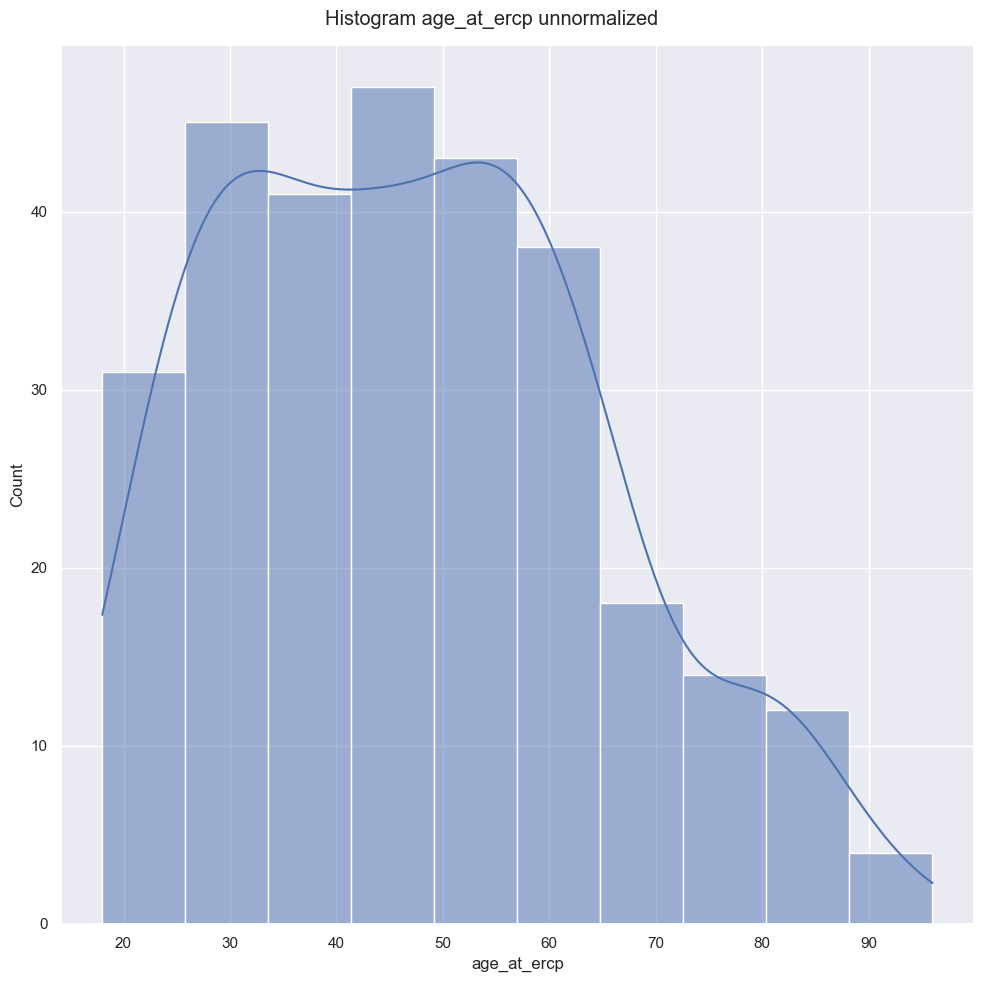
\includegraphics[width=\textwidth]{histogram_age_at_ercp_unnormalized}
		\caption{Histograma de atributo \emph{age\_at\_ercp} sin normalizar.}
	\end{subfigure}
	\hfill
	\begin{subfigure}[b]{0.4\textwidth}
		\centering
		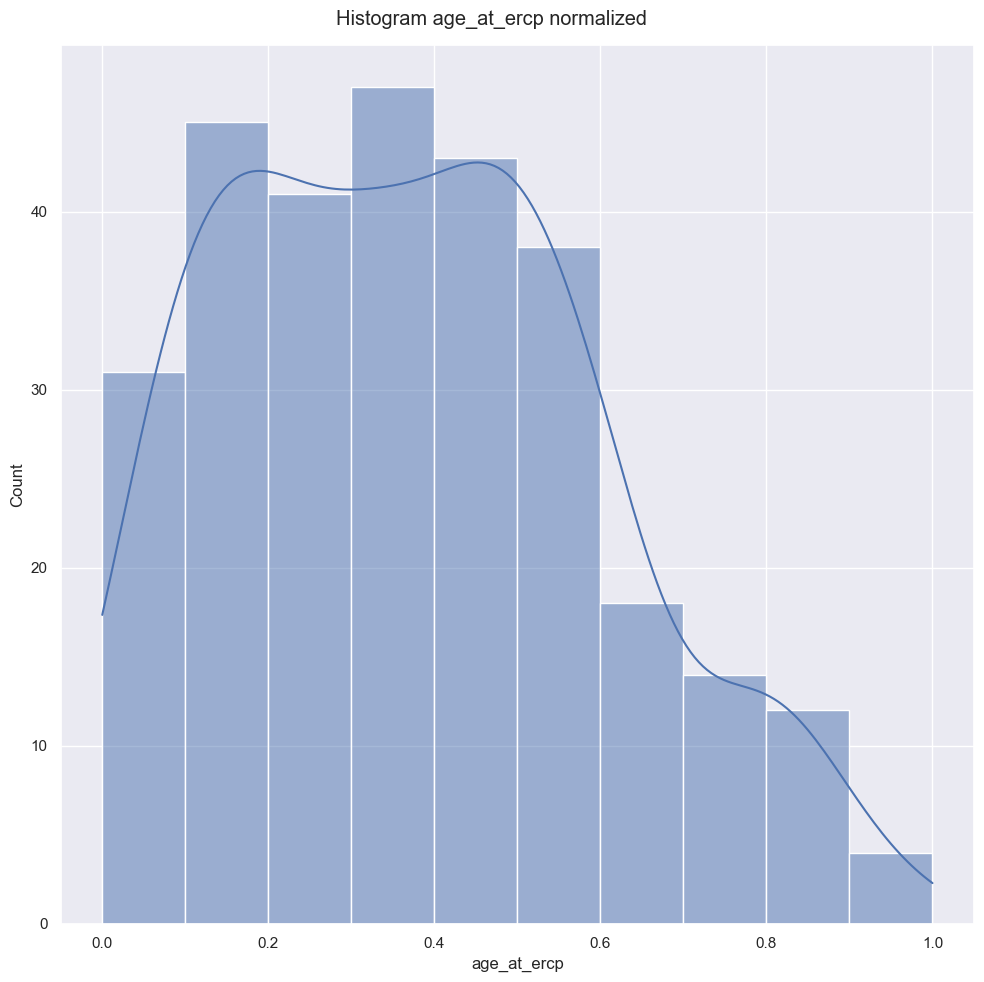
\includegraphics[width=\textwidth]{histogram_age_at_ercp_normalized}
		\caption{Histograma de atributo \emph{age\_at\_ercp} posterior a normalización.}
	\end{subfigure}
	\caption{Resultados de normalización de atributo \emph{age\_at\_ercp}}
	\label{Fig: age_at_ercp_NORM}
\end{figure}


\begin{figure}[!htb]
	\centering
	\begin{subfigure}[b]{0.4\textwidth}
		\centering
		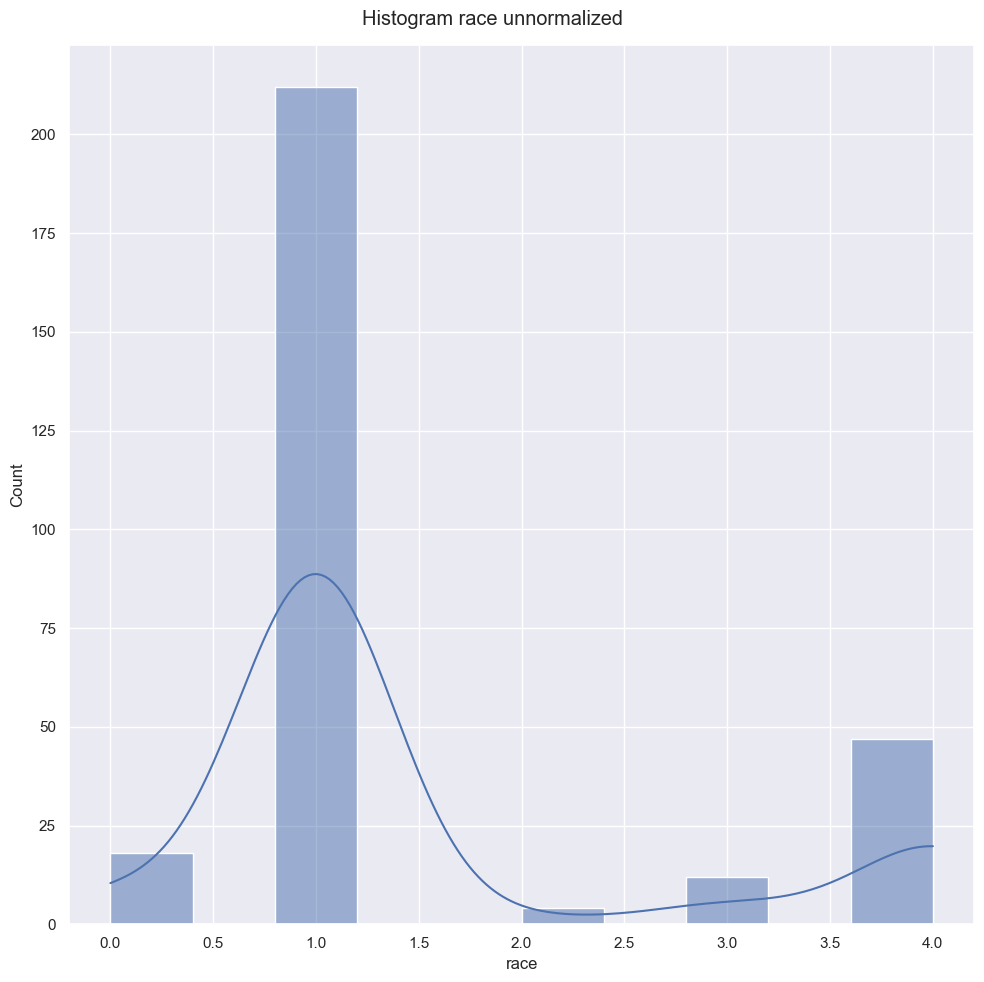
\includegraphics[width=\textwidth]{histogram_race_unnormalized}
		\caption{Histograma de atributo \emph{race} sin normalizar.}
	\end{subfigure}
	\hfill
	\begin{subfigure}[b]{0.4\textwidth}
		\centering
		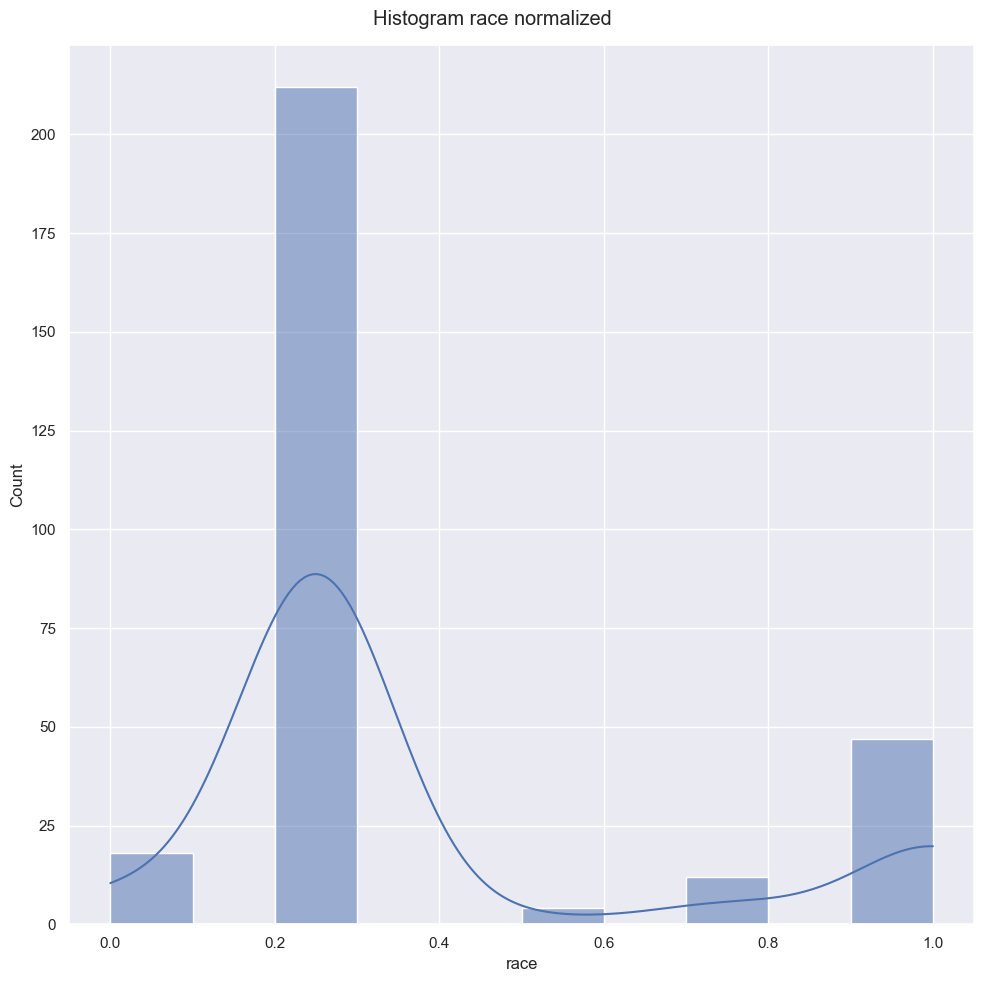
\includegraphics[width=\textwidth]{histogram_race_normalized}
		\caption{Histograma de atributo \emph{race} posterior a normalización.}
	\end{subfigure}
	\caption{Resultados de normalización de atributo \emph{race}}
	\label{Fig: race_NORM}
\end{figure}


\begin{figure}[!htb]
	\centering
	\begin{subfigure}[b]{0.4\textwidth}
		\centering
		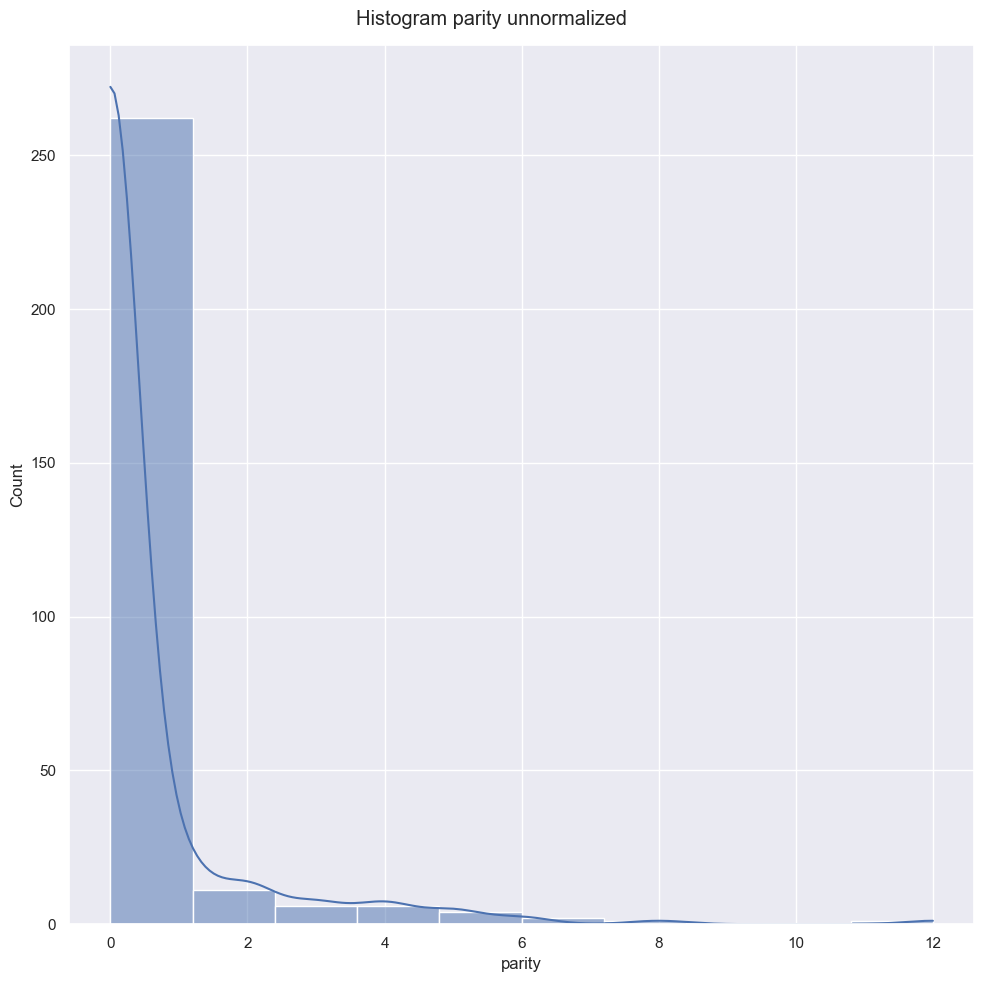
\includegraphics[width=\textwidth]{histogram_parity_unnormalized}
		\caption{Histograma de atributo \emph{parity} sin normalizar.}
	\end{subfigure}
	\hfill
	\begin{subfigure}[b]{0.4\textwidth}
		\centering
		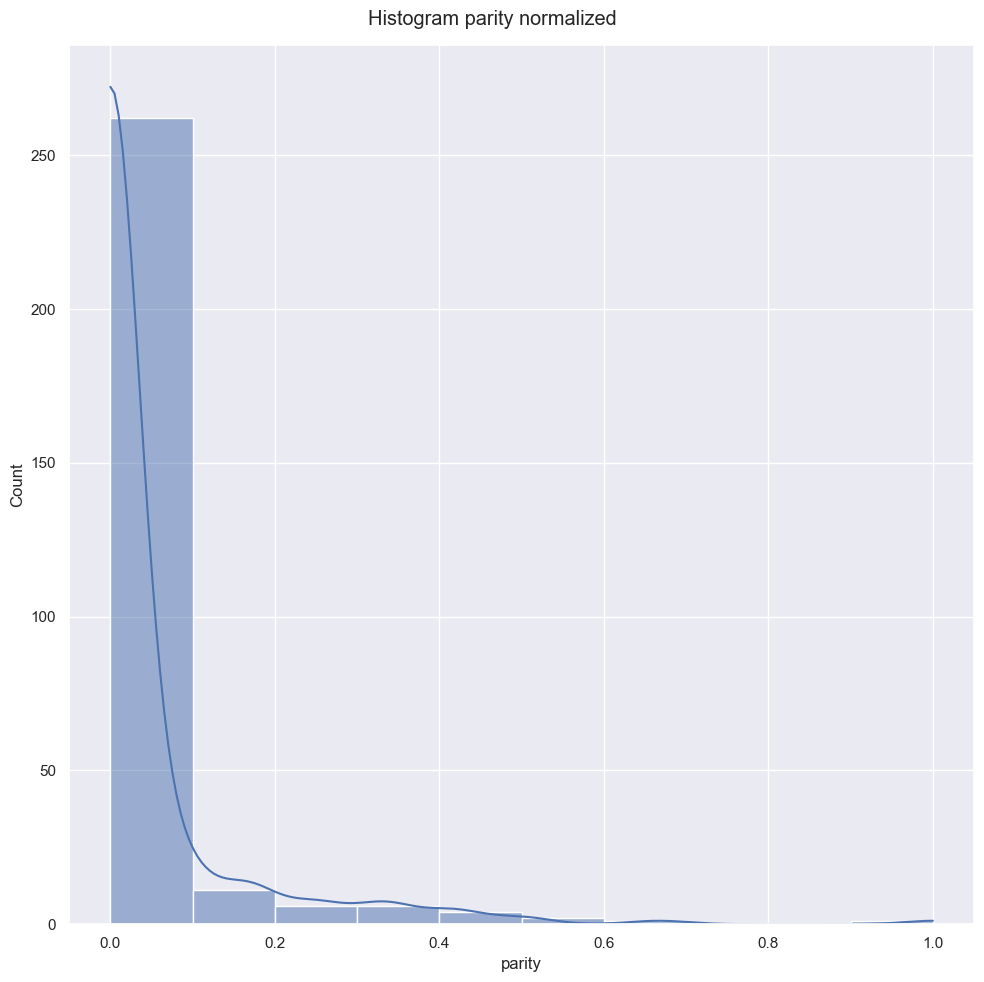
\includegraphics[width=\textwidth]{histogram_parity_normalized}
		\caption{Histograma de atributo \emph{parity} posterior a normalización.}
	\end{subfigure}
	\caption{Resultados de normalización de atributo \emph{parity}}
	\label{Fig: parity_NORM}
\end{figure}


\begin{figure}[!htb]
	\centering
	\begin{subfigure}[b]{0.4\textwidth}
		\centering
		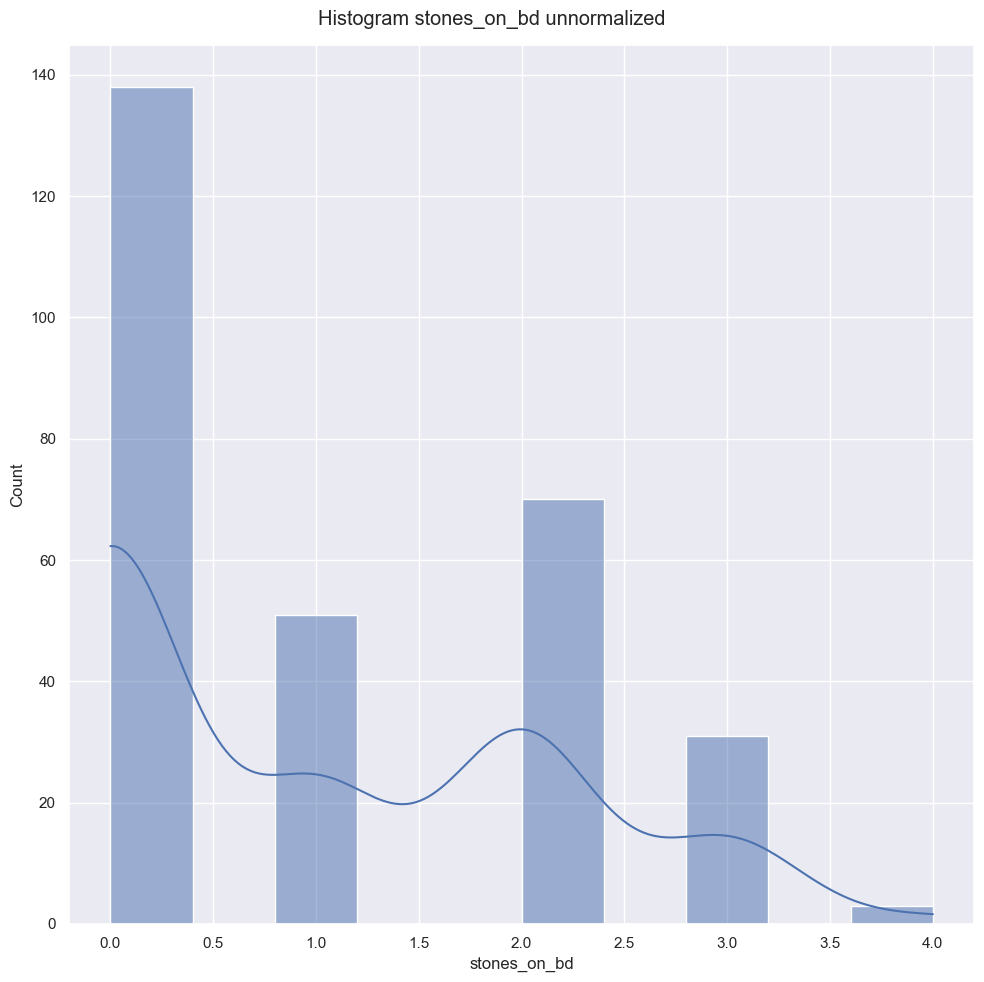
\includegraphics[width=\textwidth]{histogram_stones_on_bd_unnormalized}
		\caption{Histograma de atributo \emph{stones\_on\_bd} sin normalizar.}
	\end{subfigure}
	\hfill
	\begin{subfigure}[b]{0.4\textwidth}
		\centering
		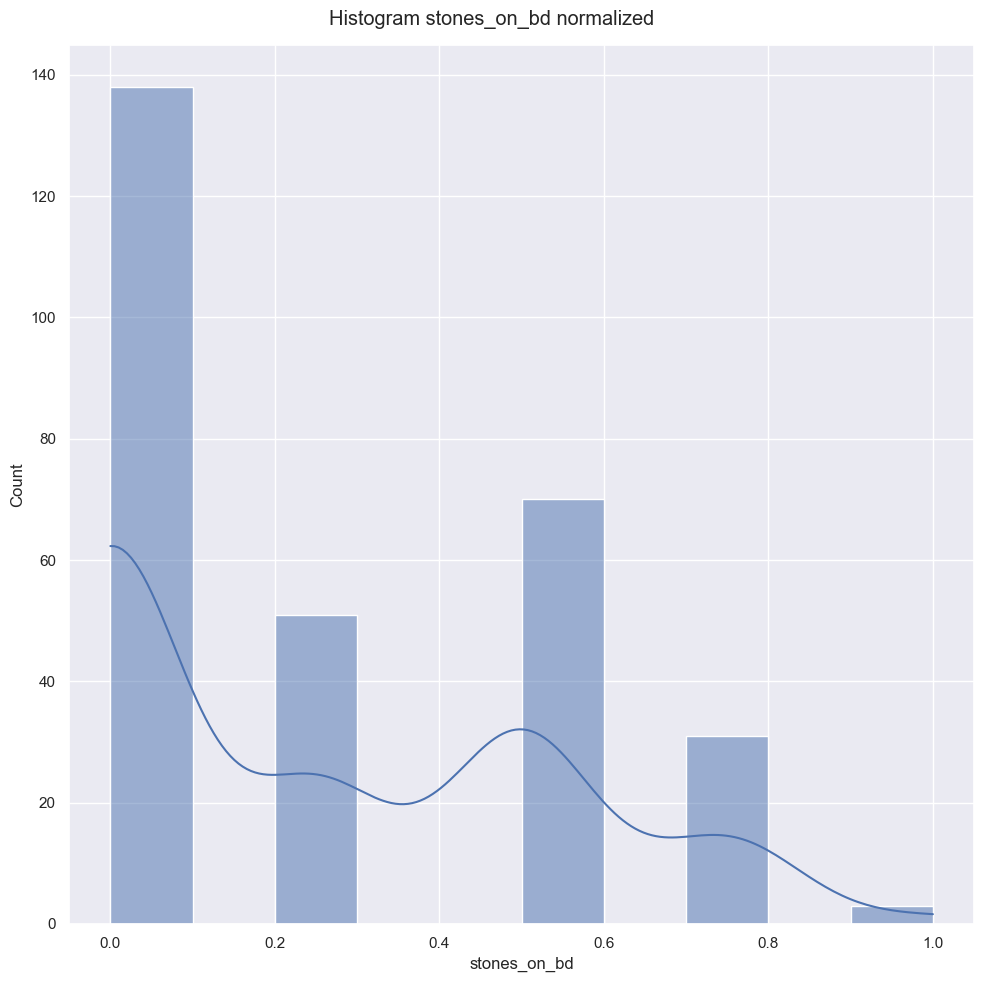
\includegraphics[width=\textwidth]{histogram_stones_on_bd_normalized}
		\caption{Histograma de atributo \emph{stones\_on\_bd} posterior a normalización.}
	\end{subfigure}
	\caption{Resultados de normalización de atributo \emph{stones\_on\_bd}}
	\label{Fig: stones_on_bd_NORM}
\end{figure}


\begin{figure}[!htb]
	\centering
	\begin{subfigure}[b]{0.4\textwidth}
		\centering
		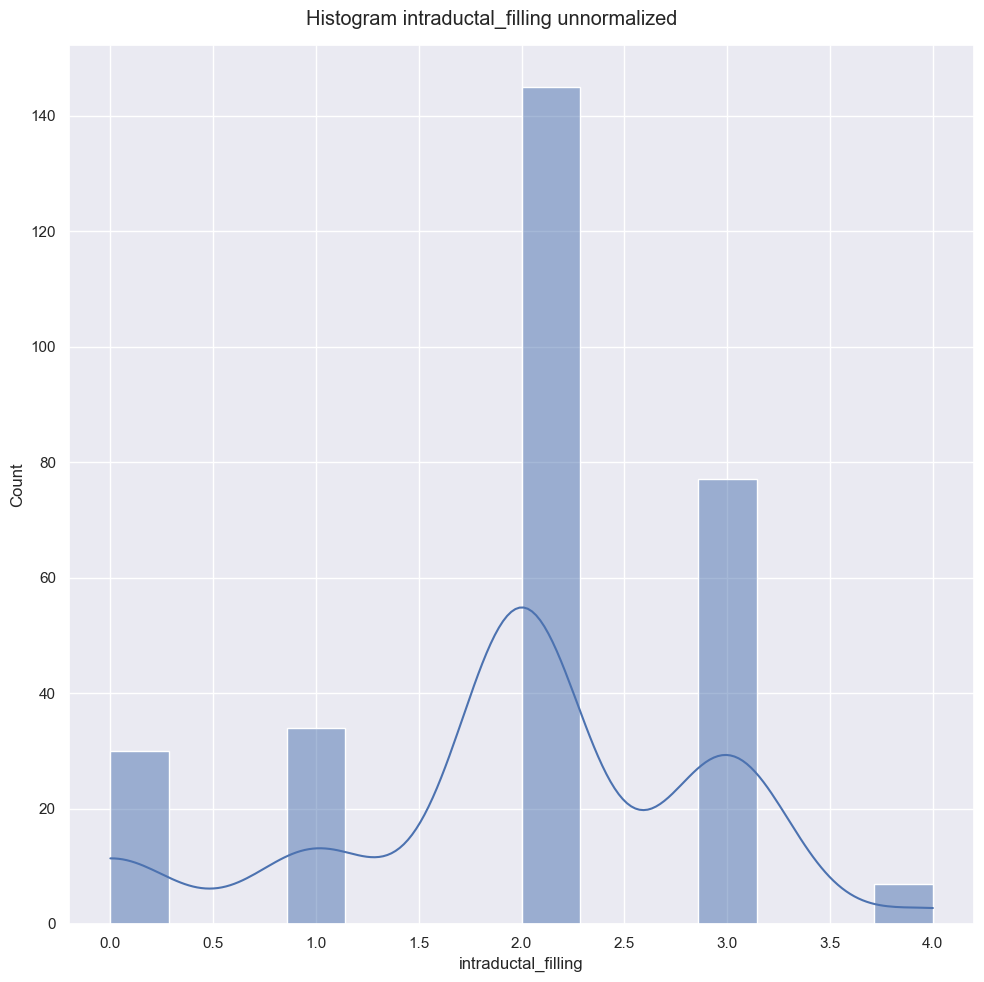
\includegraphics[width=\textwidth]{histogram_intraductal_filling_unnormalized}
		\caption{Histograma de atributo \emph{intraductal\_filling} sin normalizar.}
	\end{subfigure}
	\hfill
	\begin{subfigure}[b]{0.4\textwidth}
		\centering
		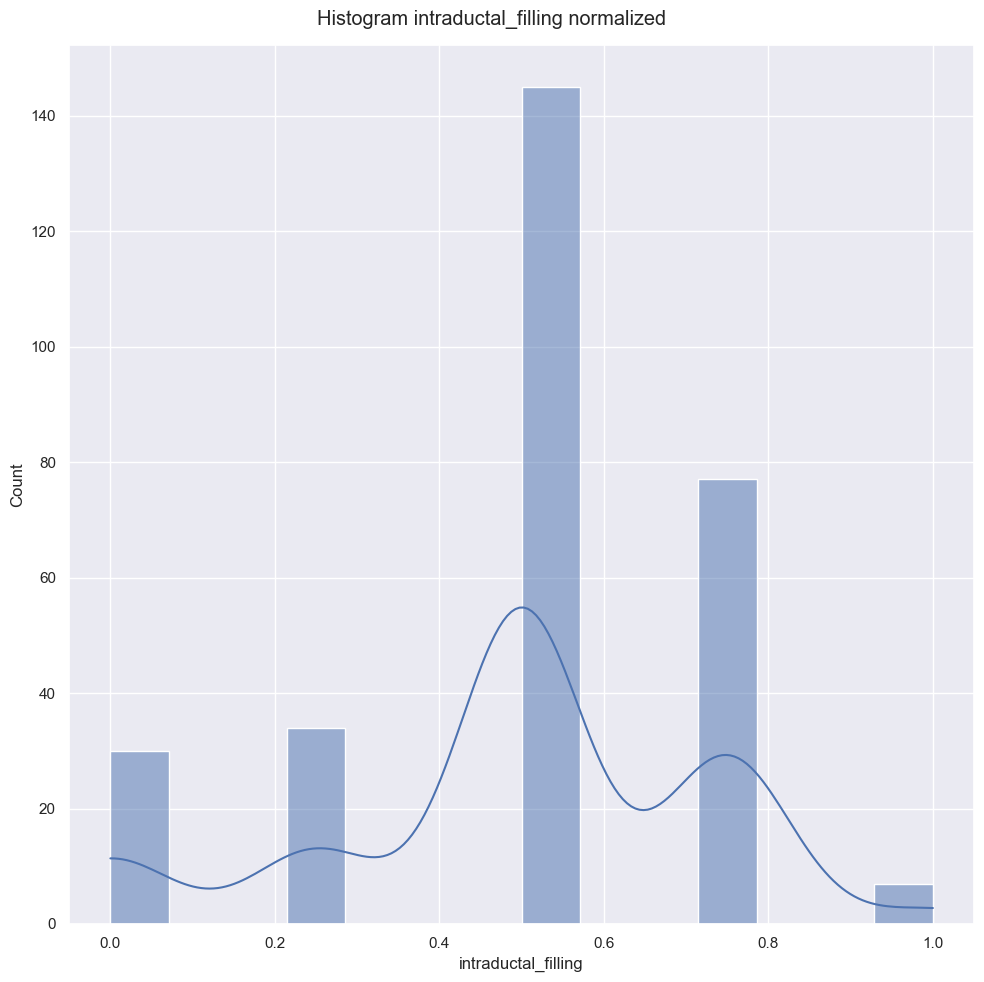
\includegraphics[width=\textwidth]{histogram_intraductal_filling_normalized}
		\caption{Histograma de atributo \emph{intraductal\_filling} posterior a normalización.}
	\end{subfigure}
	\caption{Resultados de normalización de atributo \emph{intraductal\_filling}}
	\label{Fig: intraductal_filling_NORM}
\end{figure}


\begin{figure}[!htb]
	\centering
	\begin{subfigure}[b]{0.4\textwidth}
		\centering
		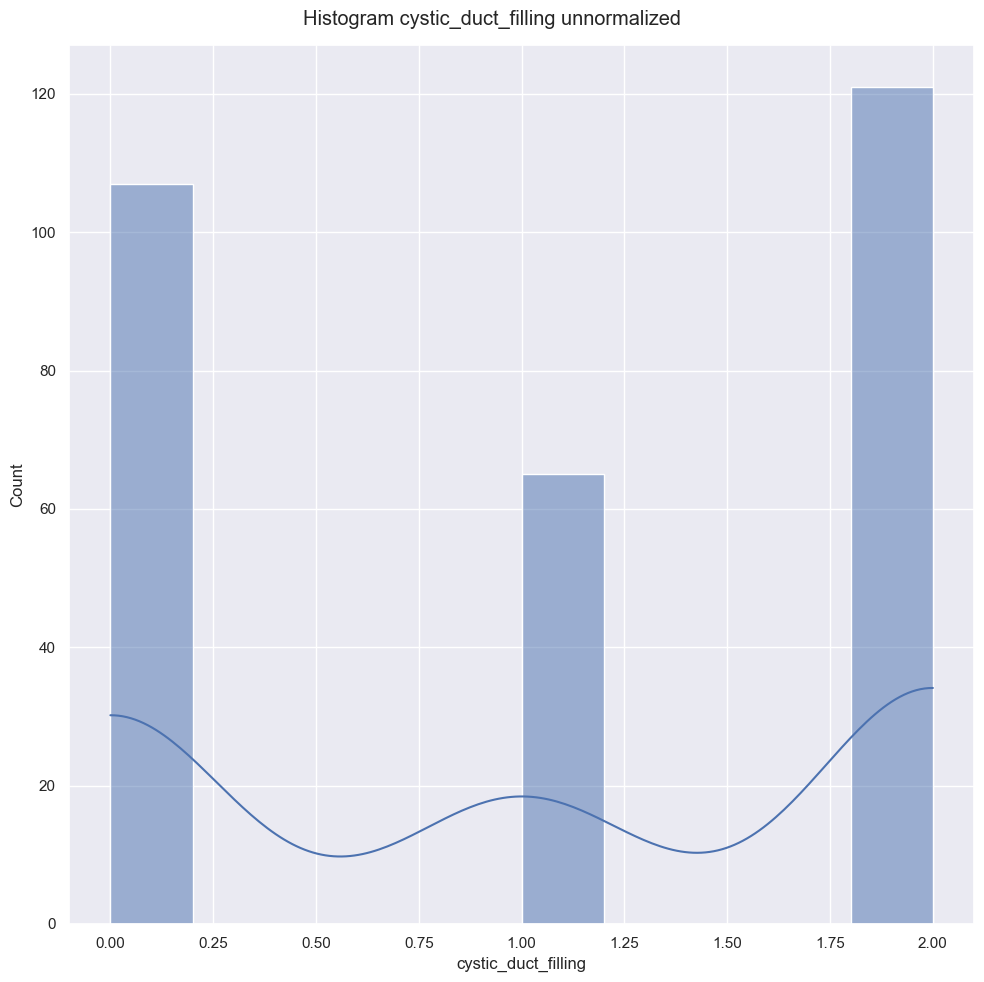
\includegraphics[width=\textwidth]{histogram_cystic_duct_filling_unnormalized}
		\caption{Histograma de atributo \emph{cystic\_duct\_filling} sin normalizar.}
	\end{subfigure}
	\hfill
	\begin{subfigure}[b]{0.4\textwidth}
		\centering
		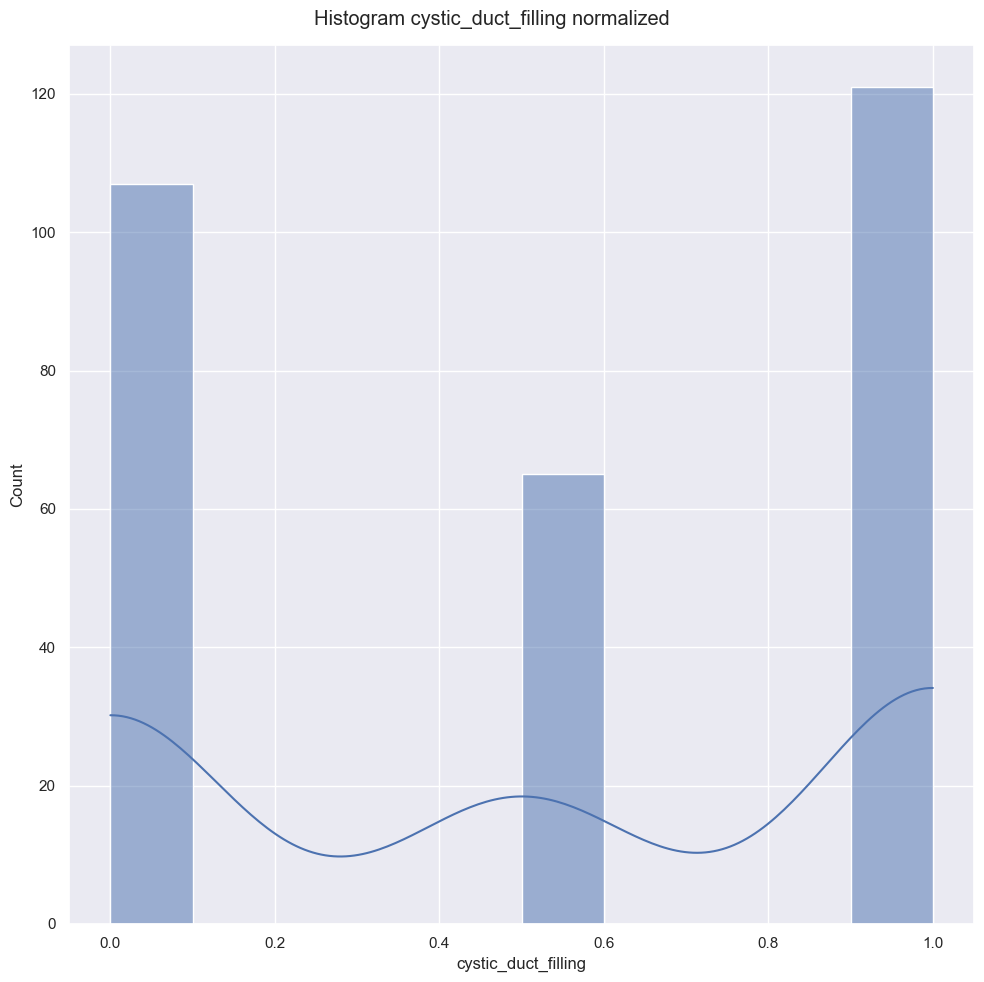
\includegraphics[width=\textwidth]{histogram_cystic_duct_filling_normalized}
		\caption{Histograma de atributo \emph{cystic\_duct\_filling} posterior a normalización.}
	\end{subfigure}
	\caption{Resultados de normalización de atributo \emph{cystic\_duct\_filling}}
	\label{Fig: cystic_duct_filling_NORM}
\end{figure}


\FloatBarrier
\subsubsection{Normalización z-score}
La Figuras \ref{Fig: bmi_NORM} - \ref{Fig: cbd_diameter_ercp_NORM} muestran los resultados de normalización de los atributos elegidos para el método z-score.

\begin{figure}[!htb]
	\centering
	\begin{subfigure}[b]{0.4\textwidth}
		\centering
		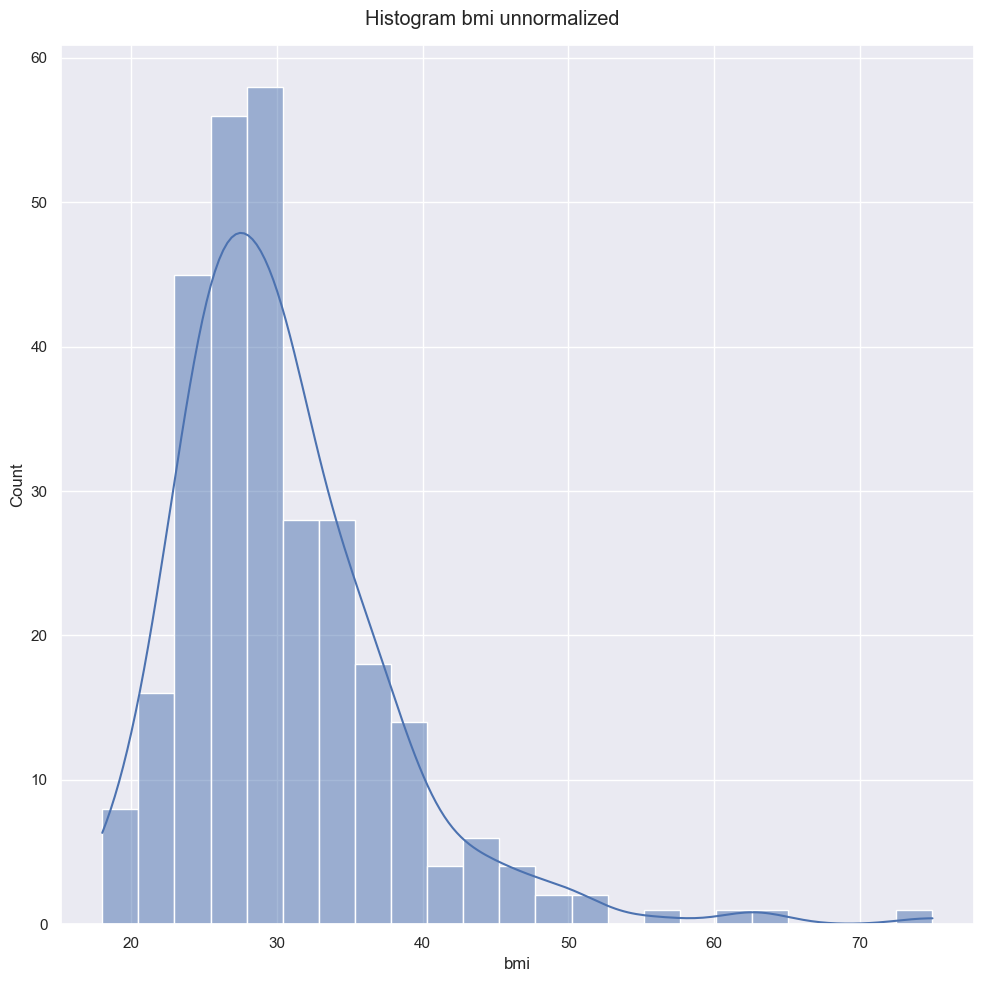
\includegraphics[width=\textwidth]{histogram_bmi_unnormalized}
		\caption{Histograma de atributo \emph{bmi} sin normalizar.}
	\end{subfigure}
	\hfill
	\begin{subfigure}[b]{0.4\textwidth}
		\centering
		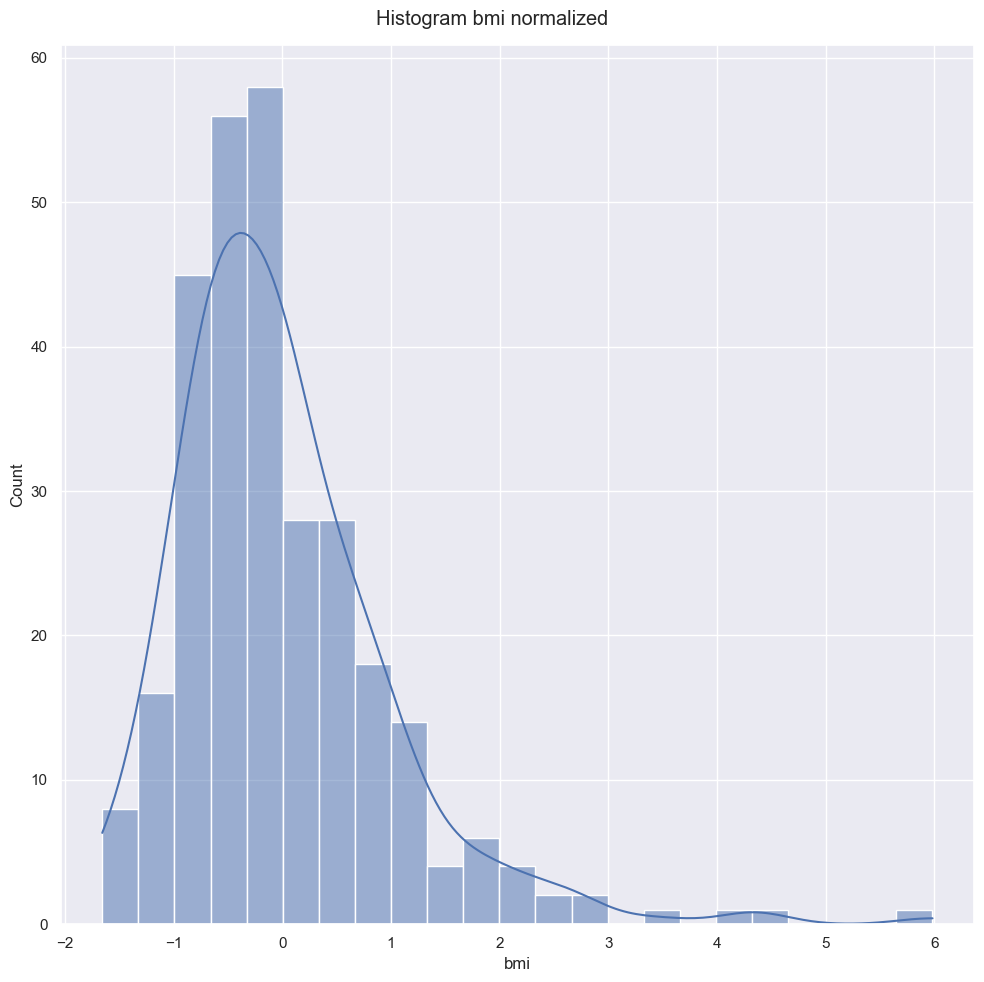
\includegraphics[width=\textwidth]{histogram_bmi_normalized}
		\caption{Histograma de atributo \emph{bmi} posterior a normalización.}
	\end{subfigure}
	\caption{Resultados de normalización de atributo \emph{bmi}}
	\label{Fig: bmi_NORM}
\end{figure}


\begin{figure}[!htb]
	\centering
	\begin{subfigure}[b]{0.4\textwidth}
		\centering
		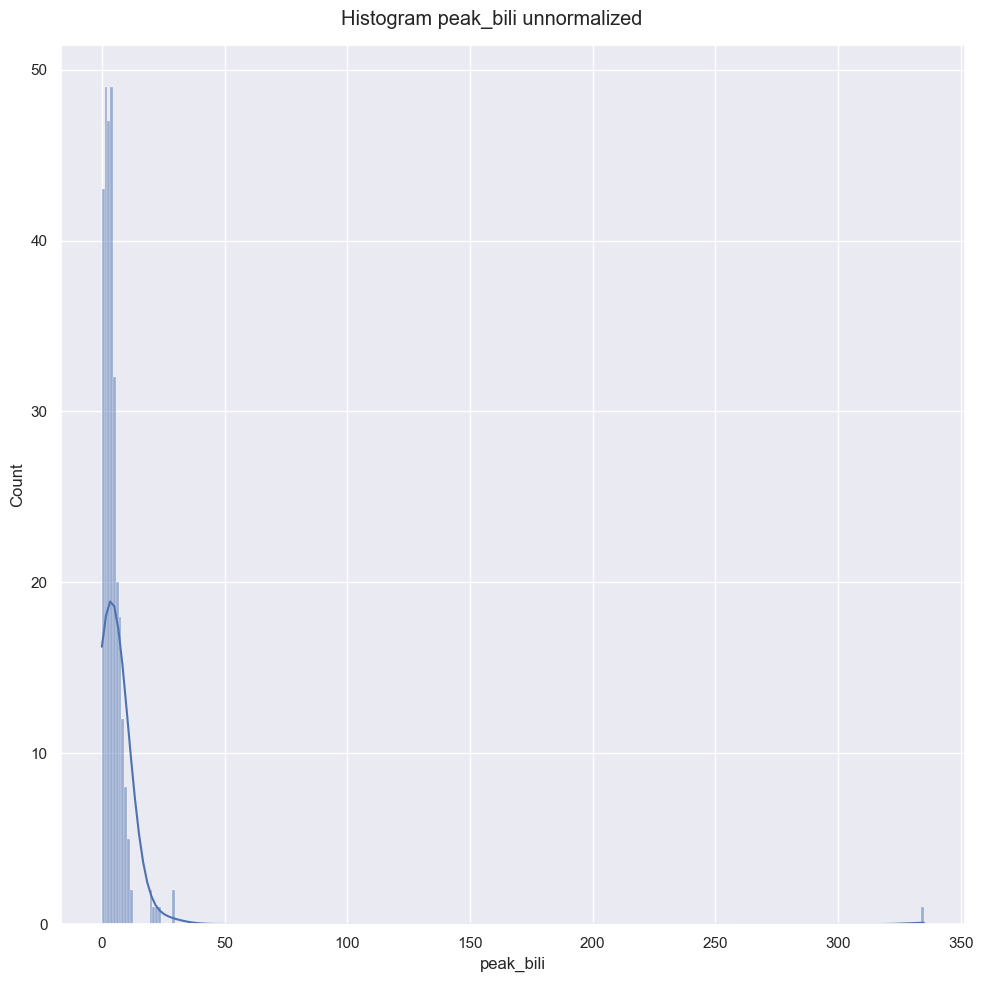
\includegraphics[width=\textwidth]{histogram_peak_bili_unnormalized}
		\caption{Histograma de atributo \emph{peak\_bili} sin normalizar.}
	\end{subfigure}
	\hfill
	\begin{subfigure}[b]{0.4\textwidth}
		\centering
		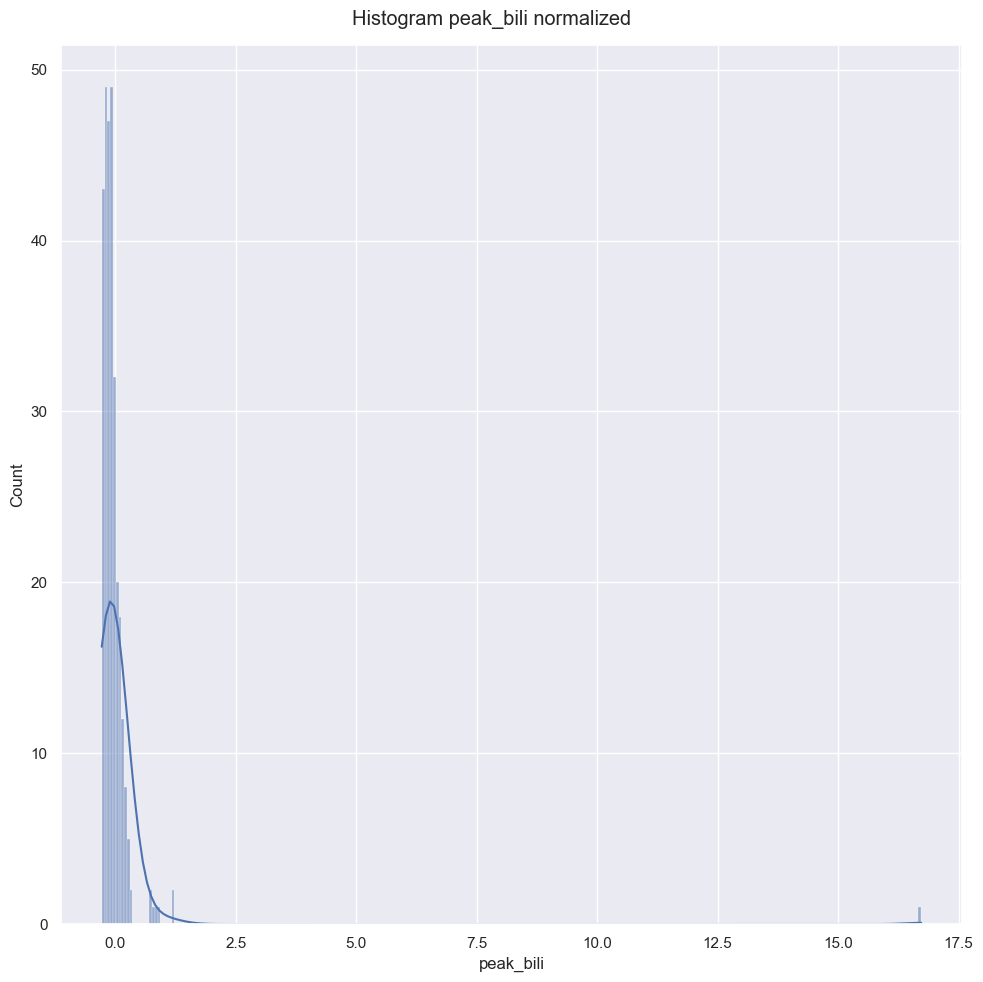
\includegraphics[width=\textwidth]{histogram_peak_bili_normalized}
		\caption{Histograma de atributo \emph{peak\_bili} posterior a normalización.}
	\end{subfigure}
	\caption{Resultados de normalización de atributo \emph{peak\_bili}}
	\label{Fig: peak_bili_NORM}
\end{figure}


\begin{figure}[!htb]
	\centering
	\begin{subfigure}[b]{0.4\textwidth}
		\centering
		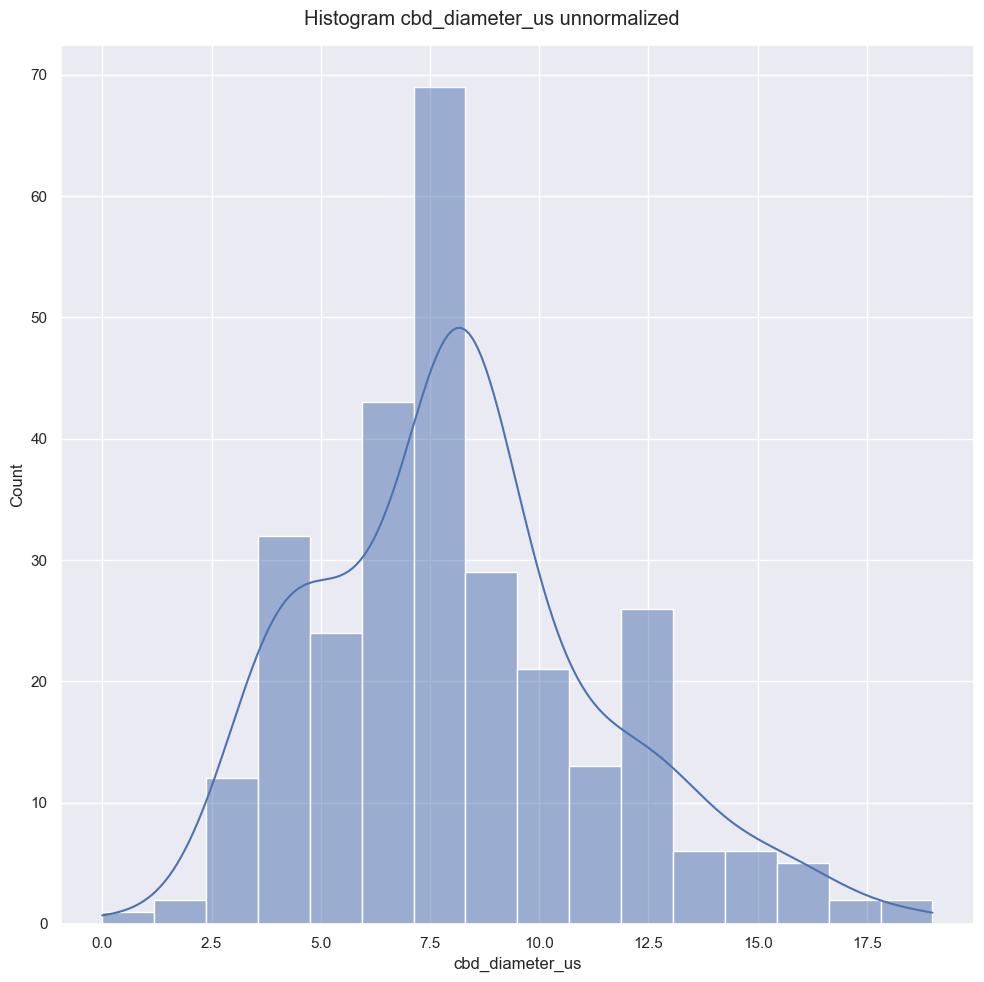
\includegraphics[width=\textwidth]{histogram_cbd_diameter_us_unnormalized}
		\caption{Histograma de atributo \emph{cbd\_diameter\_us} sin normalizar.}
	\end{subfigure}
	\hfill
	\begin{subfigure}[b]{0.4\textwidth}
		\centering
		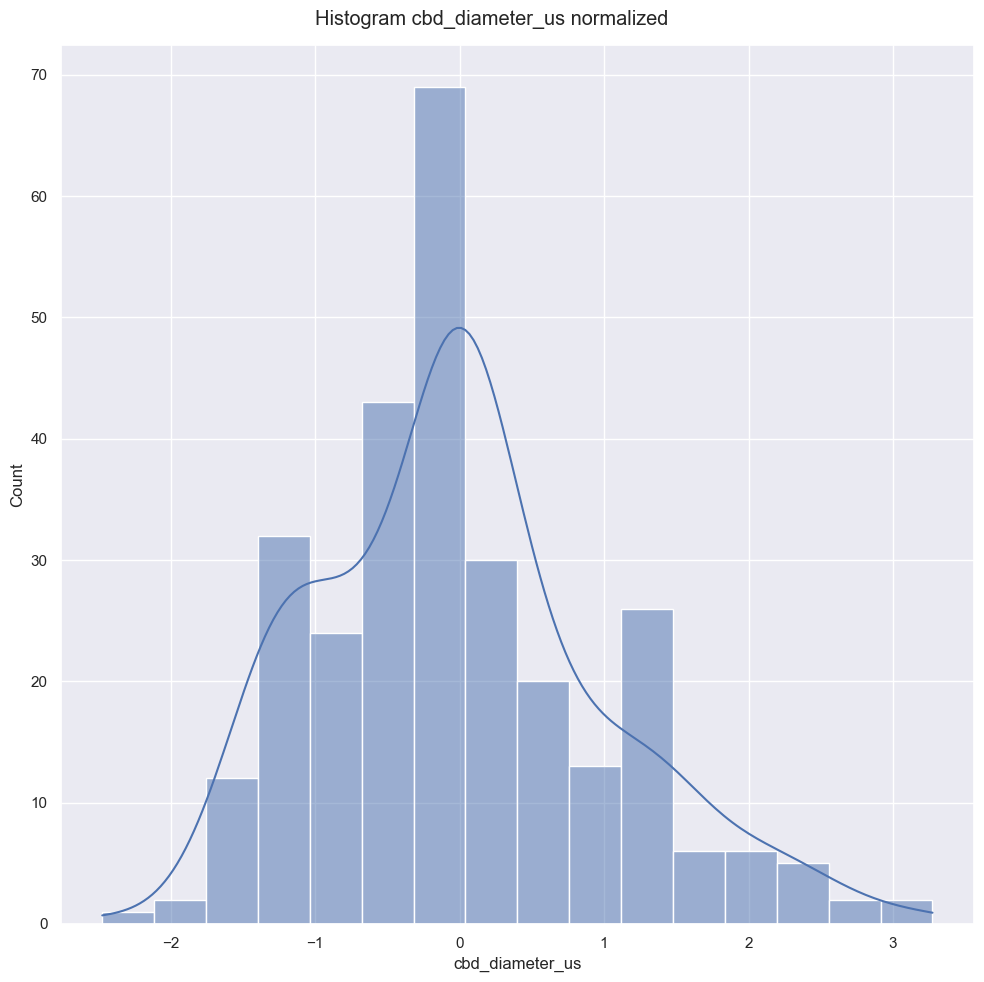
\includegraphics[width=\textwidth]{histogram_cbd_diameter_us_normalized}
		\caption{Histograma de atributo \emph{cbd\_diameter\_us} posterior a normalización.}
	\end{subfigure}
	\caption{Resultados de normalización de atributo \emph{cbd\_diameter\_us}}
	\label{Fig: cbd_diameter_us_NORM}
\end{figure}


\begin{figure}[!htb]
	\centering
	\begin{subfigure}[b]{0.4\textwidth}
		\centering
		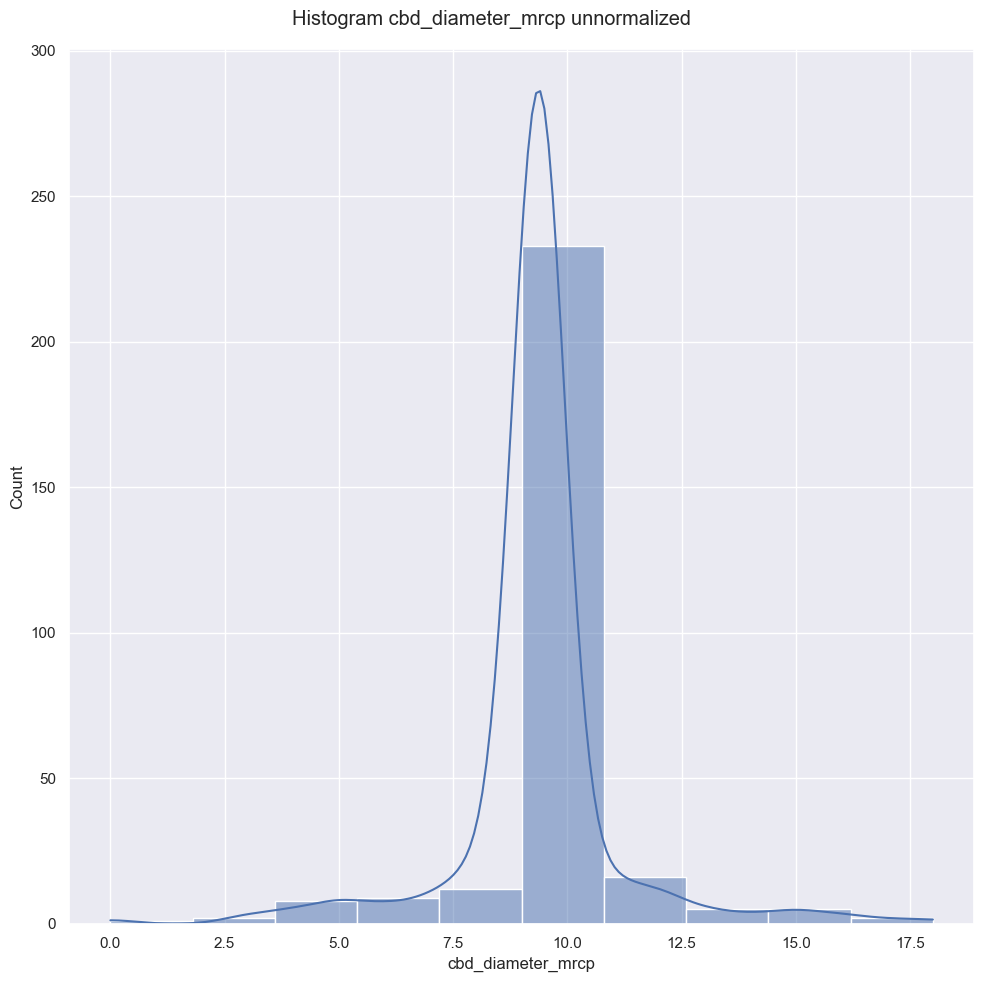
\includegraphics[width=\textwidth]{histogram_cbd_diameter_mrcp_unnormalized}
		\caption{Histograma de atributo \emph{cbd\_diameter\_mrcp} sin normalizar.}
	\end{subfigure}
	\hfill
	\begin{subfigure}[b]{0.4\textwidth}
		\centering
		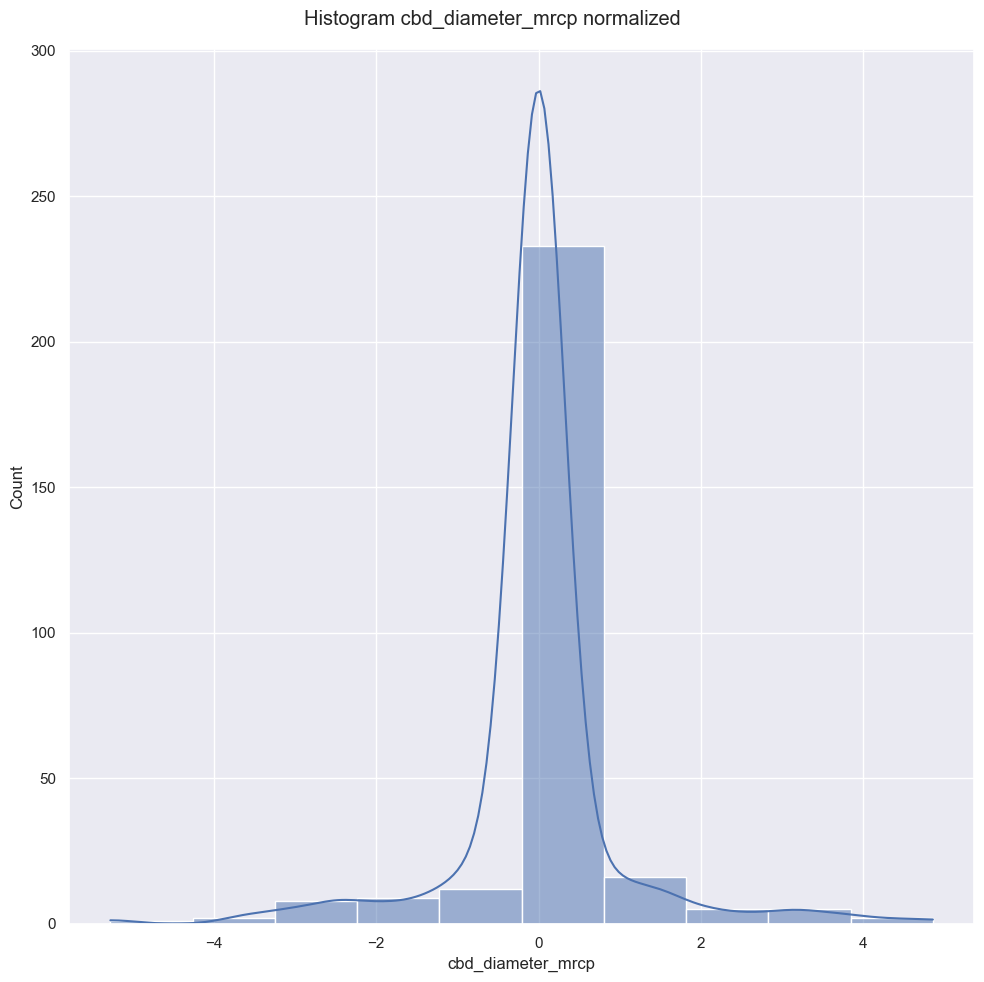
\includegraphics[width=\textwidth]{histogram_cbd_diameter_mrcp_normalized}
		\caption{Histograma de atributo \emph{cbd\_diameter\_mrcp} posterior a normalización.}
	\end{subfigure}
	\caption{Resultados de normalización de atributo \emph{cbd\_diameter\_mrcp}}
	\label{Fig: cbd_diameter_mrcp_NORM}
\end{figure}


\begin{figure}[!htb]
	\centering
	\begin{subfigure}[b]{0.4\textwidth}
		\centering
		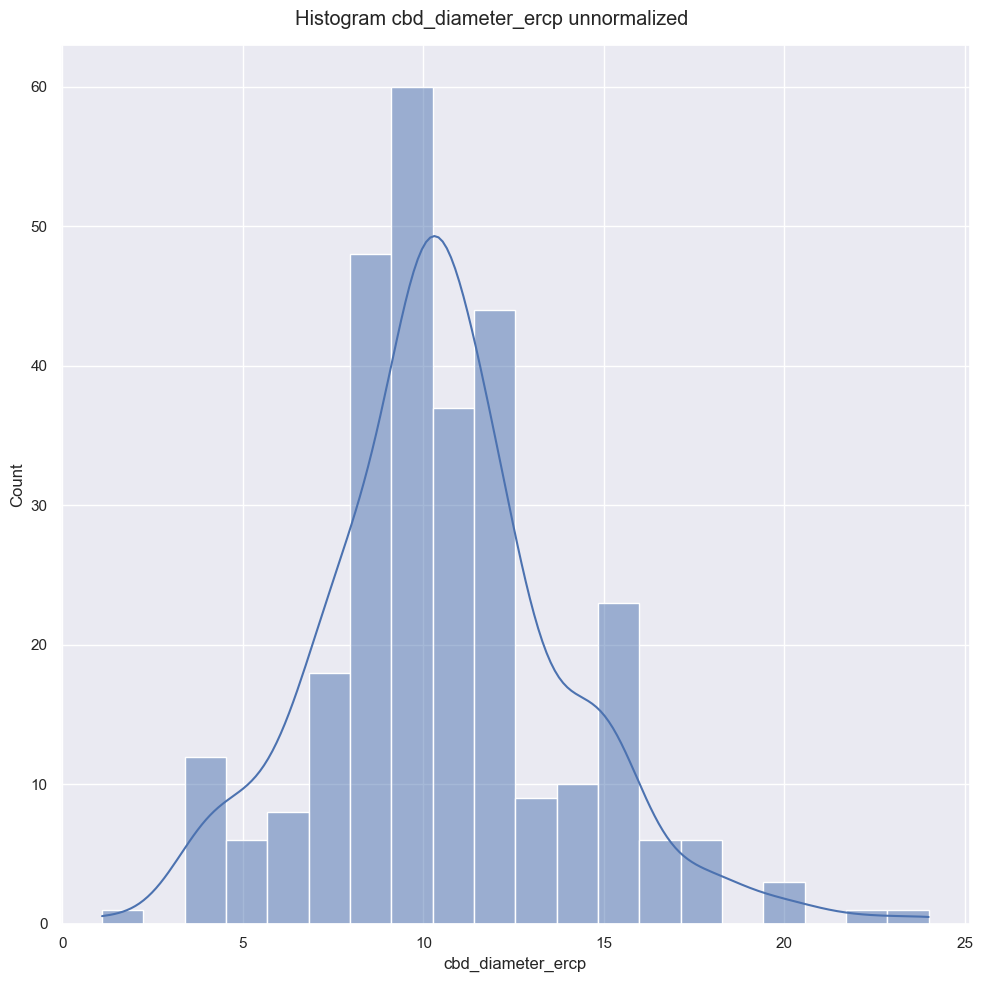
\includegraphics[width=\textwidth]{histogram_cbd_diameter_ercp_unnormalized}
		\caption{Histograma de atributo \emph{cbd\_diameter\_ercp} sin normalizar.}
	\end{subfigure}
	\hfill
	\begin{subfigure}[b]{0.4\textwidth}
		\centering
		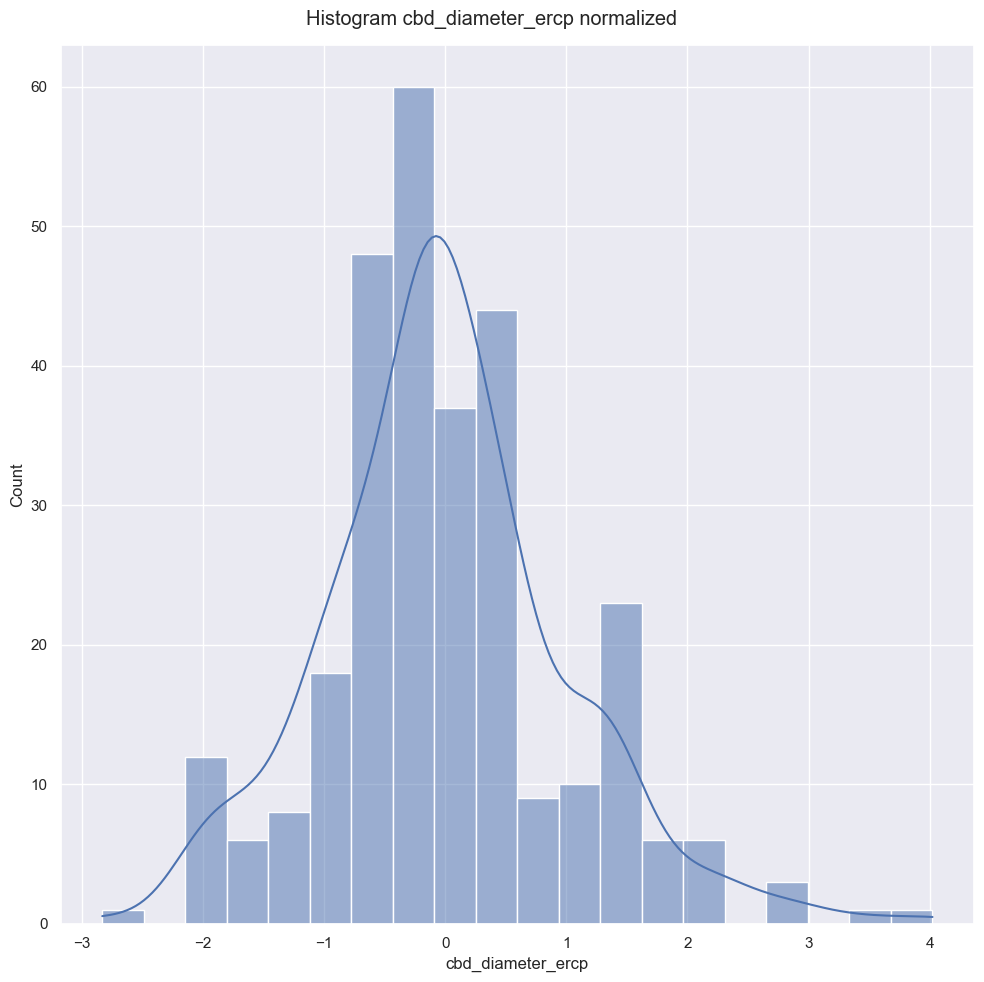
\includegraphics[width=\textwidth]{histogram_cbd_diameter_ercp_normalized}
		\caption{Histograma de atributo \emph{cbd\_diameter\_ercp} posterior a normalización.}
	\end{subfigure}
	\caption{Resultados de normalización de atributo \emph{cbd\_diameter\_mrcp}}
	\label{Fig: cbd_diameter_ercp_NORM}
\end{figure}


\FloatBarrier
\subsubsection{Normalización L1}
La Figuras \ref{Fig: pyobilia_ercp_NORM} - \ref{Fig: stone_shape_ercp_NORM} muestran los resultados de normalización de los atributos elegidos para el método L1.

\begin{figure}[!htb]
	\centering
	\begin{subfigure}[b]{0.4\textwidth}
		\centering
		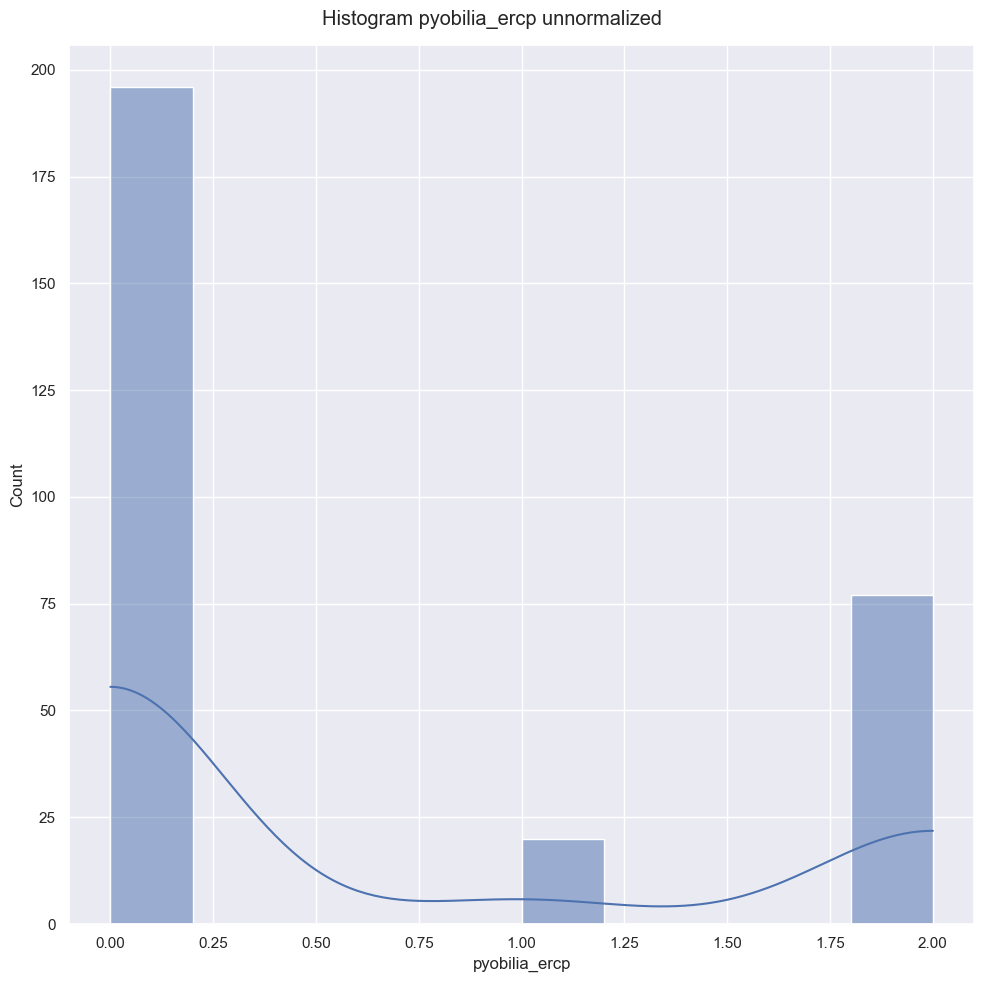
\includegraphics[width=\textwidth]{histogram_pyobilia_ercp_unnormalized}
		\caption{Histograma de atributo \emph{pyobilia\_ercp} sin normalizar.}
	\end{subfigure}
	\hfill
	\begin{subfigure}[b]{0.4\textwidth}
		\centering
		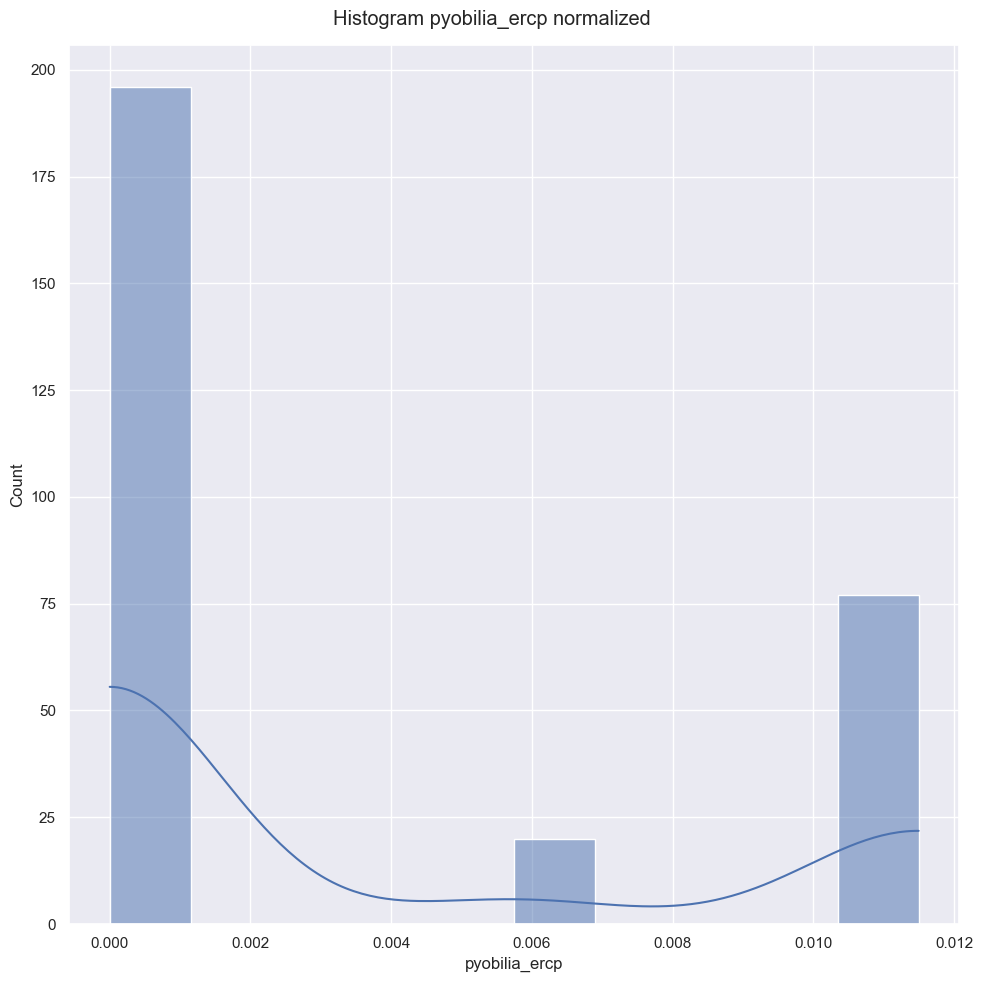
\includegraphics[width=\textwidth]{histogram_pyobilia_ercp_normalized}
		\caption{Histograma de atributo \emph{pyobilia\_ercp} posterior a normalización.}
	\end{subfigure}
	\caption{Resultados de normalización de atributo \emph{pyobilia\_ercp}}
	\label{Fig: pyobilia_ercp_NORM}
\end{figure}


\begin{figure}[!htb]
	\centering
	\begin{subfigure}[b]{0.4\textwidth}
		\centering
		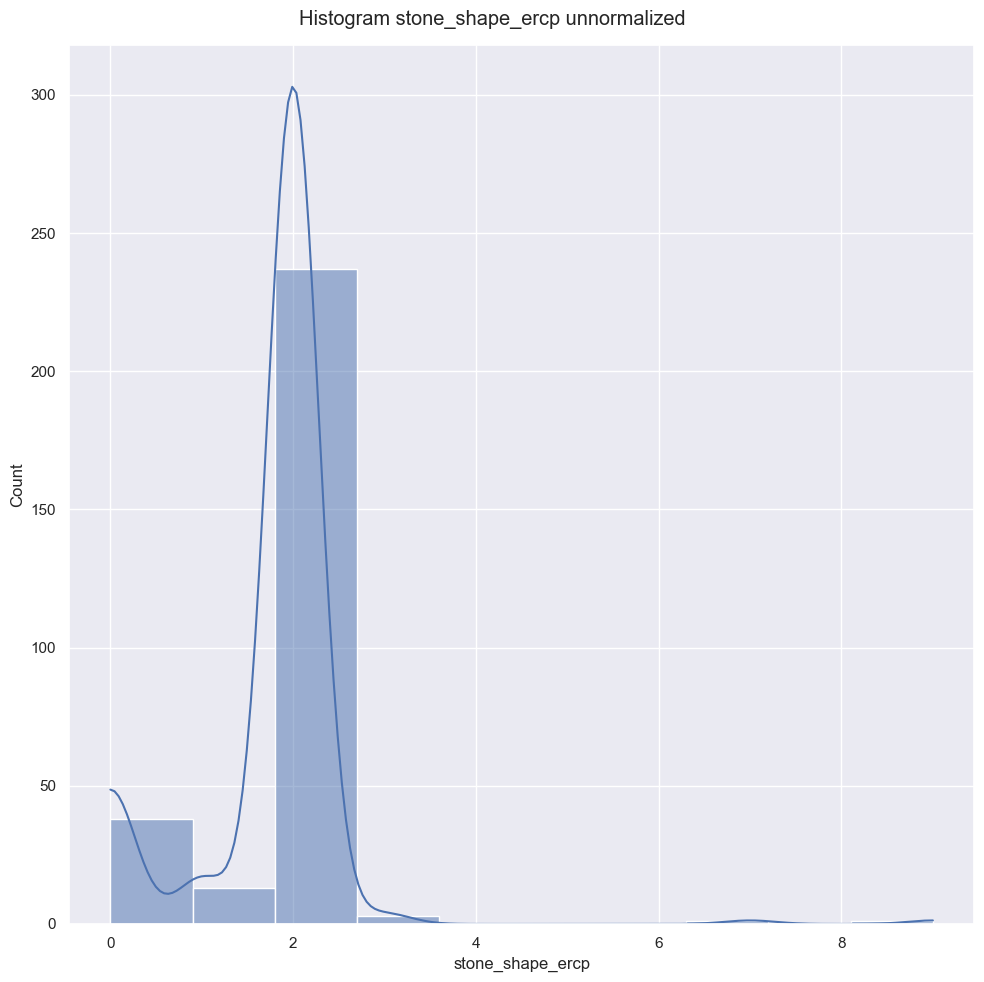
\includegraphics[width=\textwidth]{histogram_stone_shape_ercp_unnormalized}
		\caption{Histograma de atributo \emph{stone\_shape\_ercp} sin normalizar.}
	\end{subfigure}
	\hfill
	\begin{subfigure}[b]{0.4\textwidth}
		\centering
		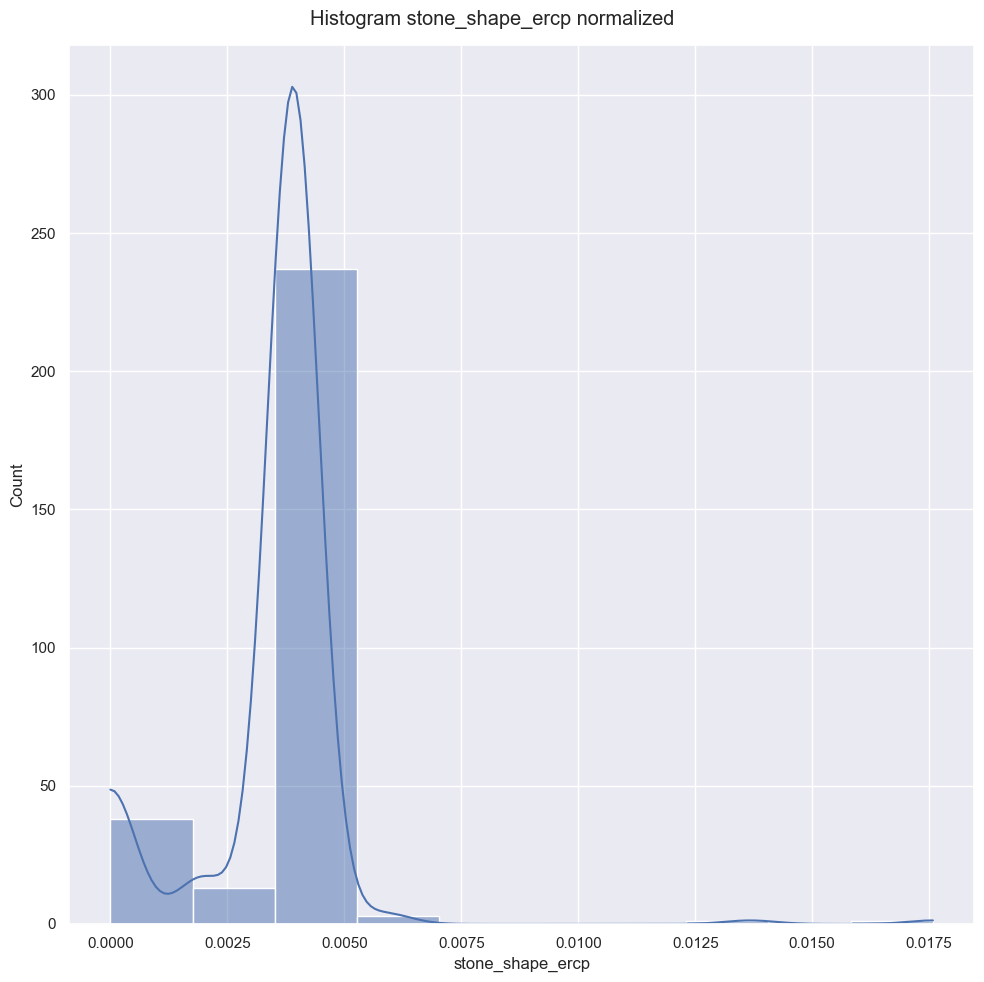
\includegraphics[width=\textwidth]{histogram_stone_shape_ercp_normalized}
		\caption{Histograma de atributo \emph{stone\_shape\_ercp} posterior a normalización.}
	\end{subfigure}
	\caption{Resultados de normalización de atributo \emph{stone\_shape\_ercp}}
	\label{Fig: stone_shape_ercp_NORM}
\end{figure}


\begin{figure}[!htb]
	\centering
	\begin{subfigure}[b]{0.4\textwidth}
		\centering
		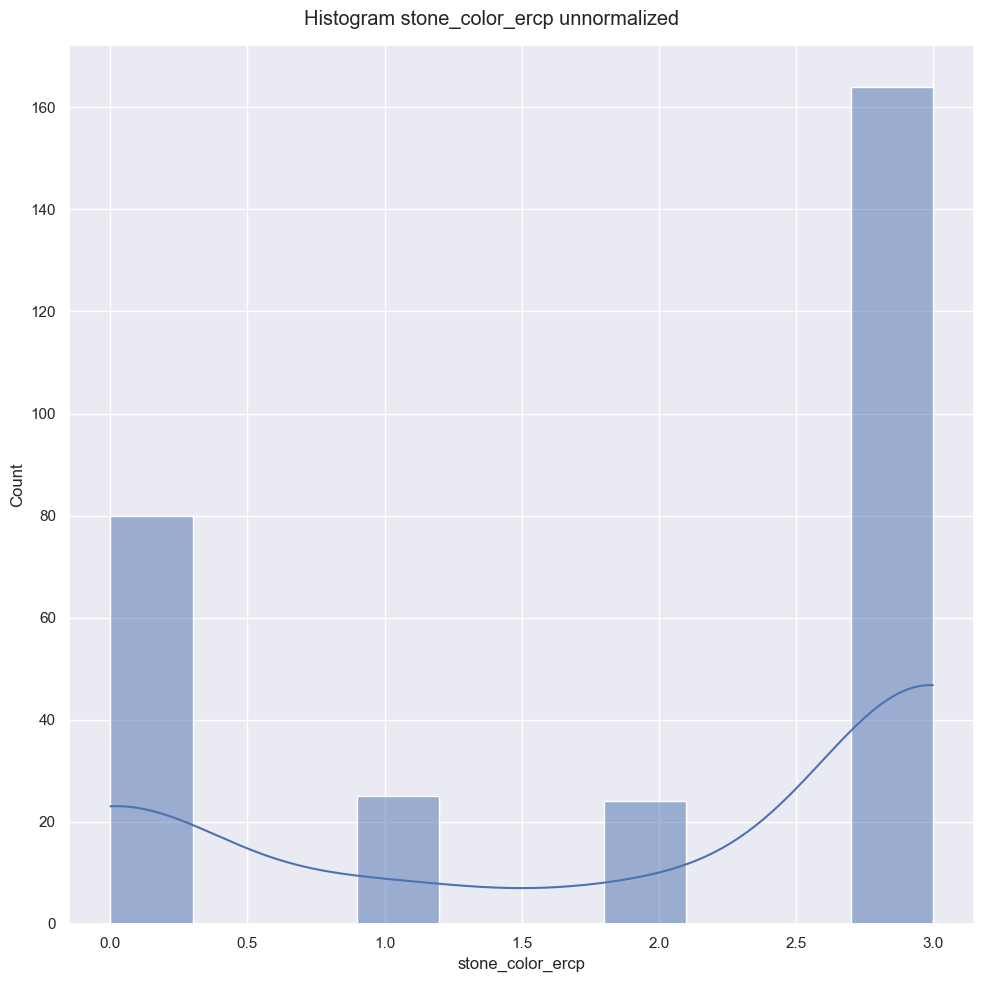
\includegraphics[width=\textwidth]{histogram_stone_color_ercp_unnormalized}
		\caption{Histograma de atributo \emph{stone\_color\_ercp} sin normalizar.}
	\end{subfigure}
	\hfill
	\begin{subfigure}[b]{0.4\textwidth}
		\centering
		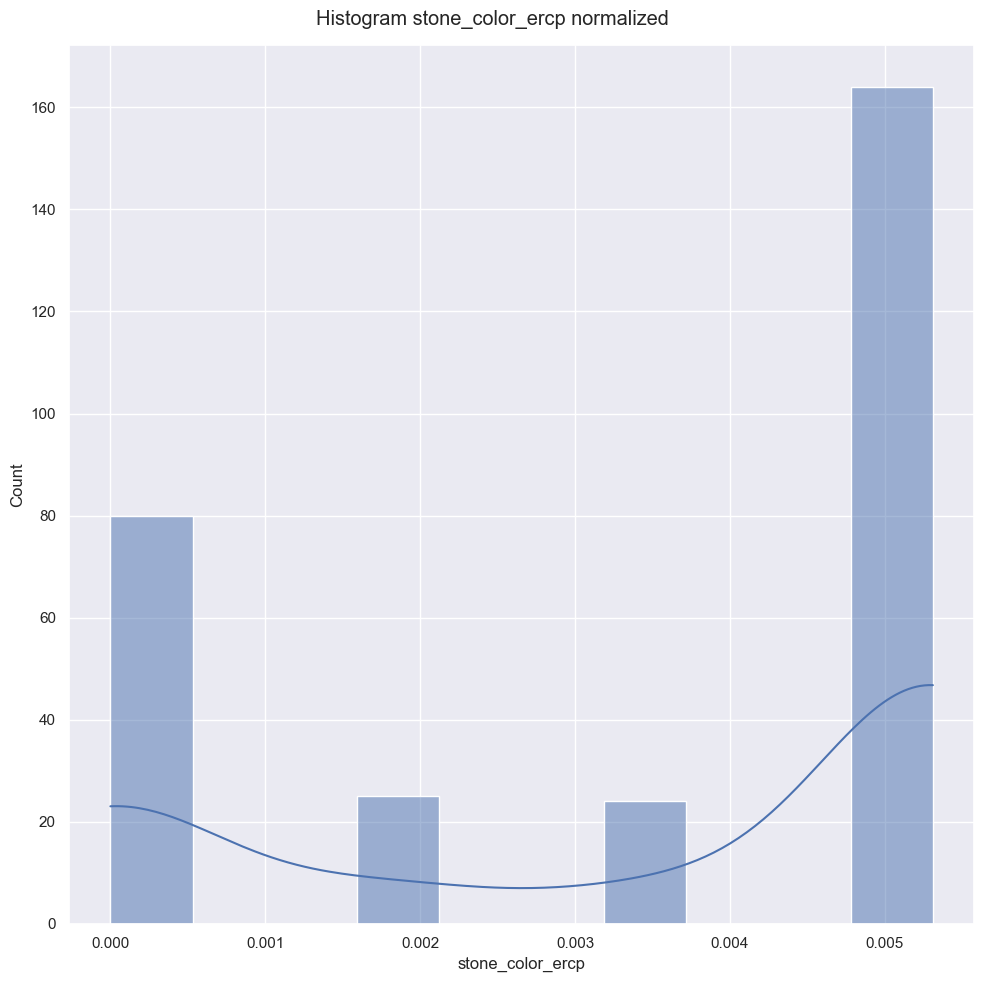
\includegraphics[width=\textwidth]{histogram_stone_color_ercp_normalized}
		\caption{Histograma de atributo \emph{stone\_color\_ercp} posterior a normalización.}
	\end{subfigure}
	\caption{Resultados de normalización de atributo \emph{stone\_shape\_ercp}}
	\label{Fig: stone_shape_ercp_NORM}
\end{figure}

%%%%%%%%%%

\FloatBarrier
\hfill \break
\subsection{Balance de clases con datos sintéticos}
La Figura \ref{Fig: original-class} muestra la distribución de clases original del conjunto de datos.

\begin{figure}[!htb]
	\centering
	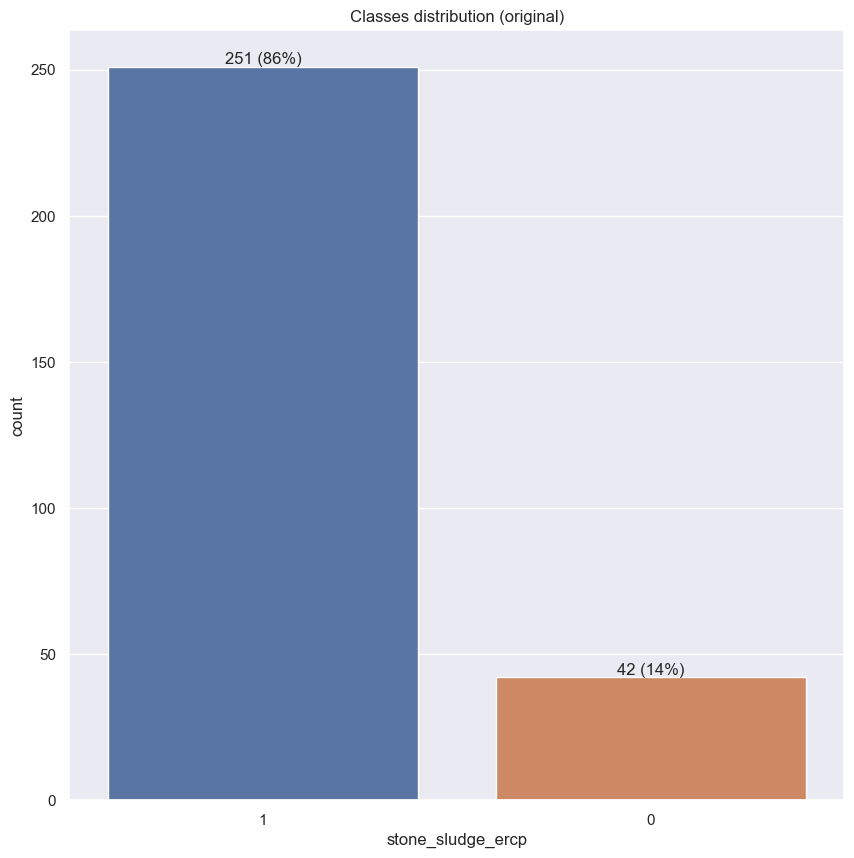
\includegraphics[width=0.7\textwidth]{classes_distribution_original}
	\caption{Distribución de clases en el conjunto de datos original}
	\label{Fig: original-class}
\end{figure}

\FloatBarrier
\subsubsection{Método de ruleta}
La Figura \ref{Fig: roulette-class} muestra la distribución de clases resultante de aplicar el método de ruleta. La Tabla \ref{Tab: Ruleta-std} muestra una comparación entre la desviación estándar de los atributos de la base datos original y los datos obtenidos tras aplicar el método ruleta. Por otro lado, la Figura \ref{Fig: roulette-hist} muestra un ejemplo de la distribución de los datos resultantes del método ruleta.

\begin{figure}[!htb]
	\centering
	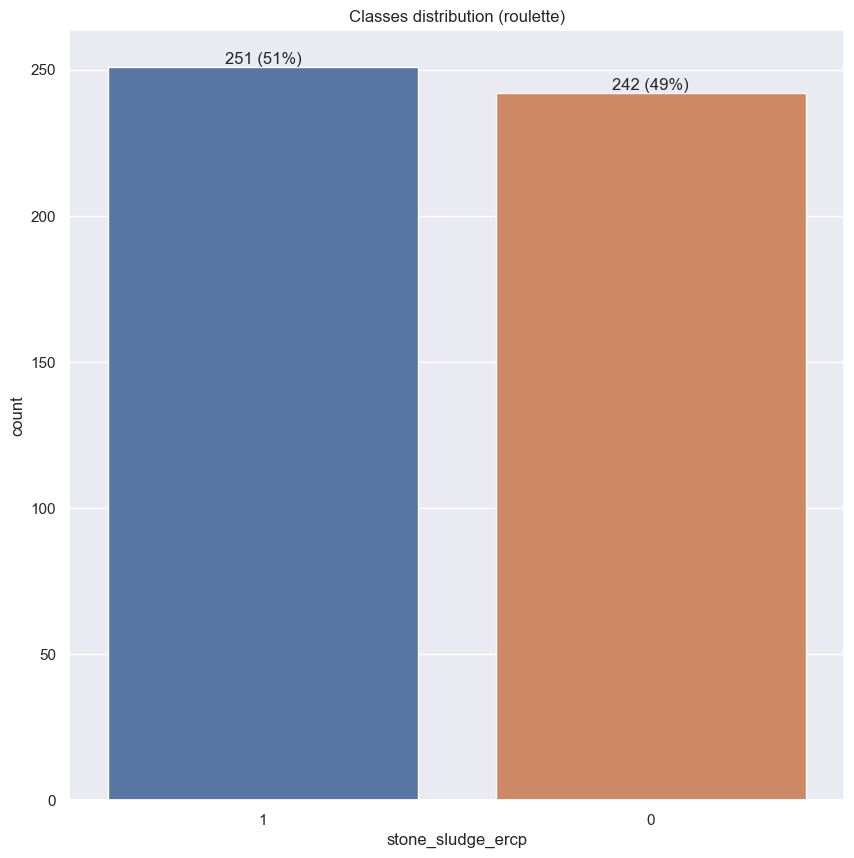
\includegraphics[width=0.7\textwidth]{classes_distribution_roulette}
	\caption{Distribución de clases en el conjunto de datos resultante del método de ruleta}
	\label{Fig: roulette-class}
\end{figure}

\begin{table}[!htb]
\centering
\caption{Comparación de los valores de desviación estándar del conjunto de datos original y posterior al balance de clases por le método de la ruleta.}
\label{Tab: Ruleta-std}
\begin{tabular}{|l|ll|}
\hline
\multicolumn{1}{|c|}{\multirow{2}{*}{\textbf{Atributo}}} & \multicolumn{2}{c|}{\textbf{$\sigma$}}                                           \\ \cline{2-3} 
\multicolumn{1}{|c|}{}                                   & \multicolumn{1}{c|}{\textbf{Original}} & \multicolumn{1}{c|}{\textbf{Ruleta}} \\ \hline
age\_at\_ercp                                            & \multicolumn{1}{l|}{17.81}             & 17.49                                \\ \hline
gender                                                   & \multicolumn{1}{l|}{0.48}              & 0.49                                 \\ \hline
race                                                     & \multicolumn{1}{l|}{1.19}              & 1.25                                 \\ \hline
bmi                                                      & \multicolumn{1}{l|}{7.47}              & 1.15                                 \\ \hline
parity                                                   & \multicolumn{1}{l|}{1.34}              & 0.46                                 \\ \hline
dm                                                       & \multicolumn{1}{l|}{0.36}              & 0.41                                 \\ \hline
ibd                                                      & \multicolumn{1}{l|}{0.05}              & 0.45                                 \\ \hline
cirrhosis                                                & \multicolumn{1}{l|}{0.18}              & 0.21                                 \\ \hline
peak\_bili                                               & \multicolumn{1}{l|}{19.73}             & 29.91                                \\ \hline
stones\_on\_bd                                           & \multicolumn{1}{l|}{1.10}              & 1.14                                 \\ \hline
cbd\_diameter\_us                                        & \multicolumn{1}{l|}{3.31}              & 3.27                                 \\ \hline
cbd\_diameter\_mrcp                                      & \multicolumn{1}{l|}{1.77}              & 1.67                                 \\ \hline
cbd\_diameter\_ercp                                      & \multicolumn{1}{l|}{3.34}              & 3.37                                 \\ \hline
intraductal\_filling                                     & \multicolumn{1}{l|}{0.94}              & 1.18                                 \\ \hline
cystic\_duct\_filling                                    & \multicolumn{1}{l|}{0.88}              & 0.92                                 \\ \hline
stone\_shape\_ercp                                       & \multicolumn{1}{l|}{0.87}              & 0.85                                 \\ \hline
stone\_color\_ercp                                       & \multicolumn{1}{l|}{1.31}              & 1.17                                 \\ \hline
pyobilia\_ercp                                           & \multicolumn{1}{l|}{0.87}              & 0.87                                 \\ \hline
gallbladder                                              & \multicolumn{1}{l|}{0.50}              & 0.53                                 \\ \hline
stone\_sludge\_ercp                                      & \multicolumn{1}{l|}{0.35}              & 0.50                                 \\ \hline
\end{tabular}
\end{table}

\begin{figure}[!htb]
	\centering
	\begin{subfigure}[b]{0.4\textwidth}
		\centering
		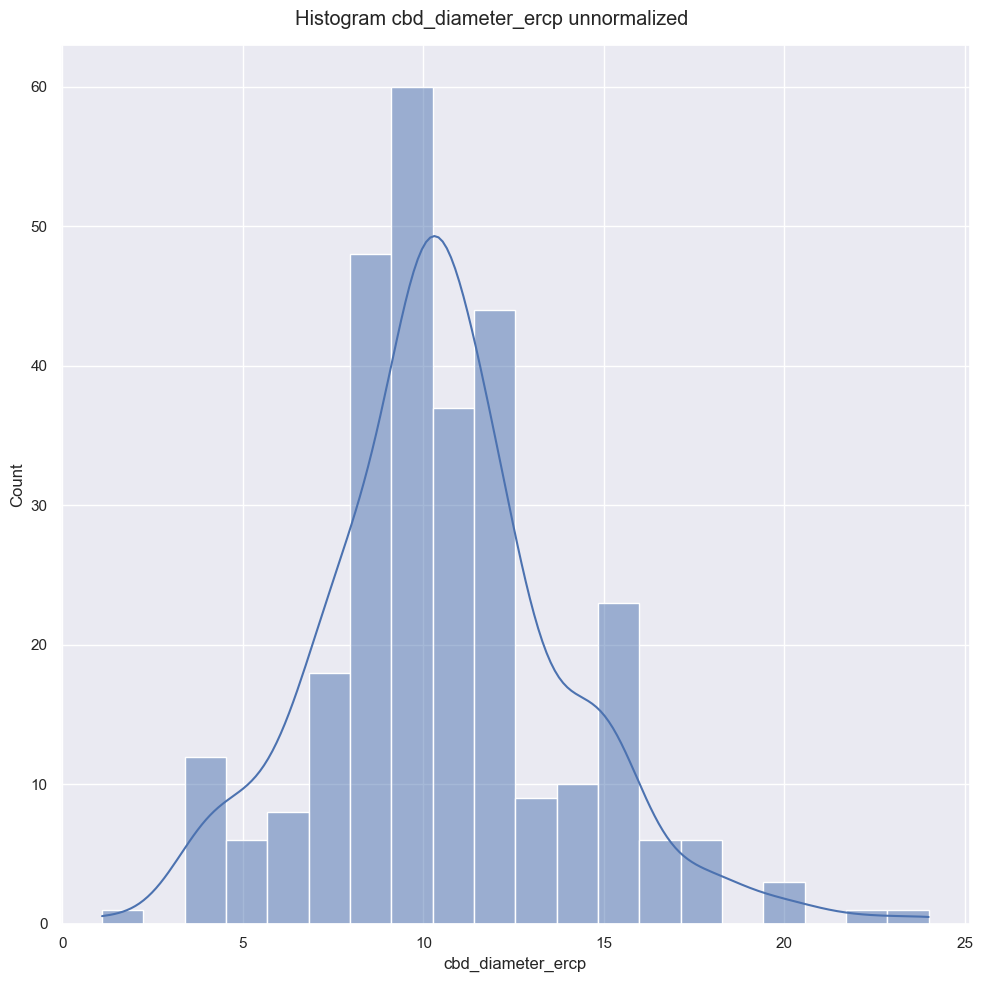
\includegraphics[width=\textwidth]{histogram_cbd_diameter_ercp_unnormalized}
		\caption{Histograma de atributo \emph{cbd\_diameter\_ercp} original.}
	\end{subfigure}
	\hfill
	\begin{subfigure}[b]{0.4\textwidth}
		\centering
		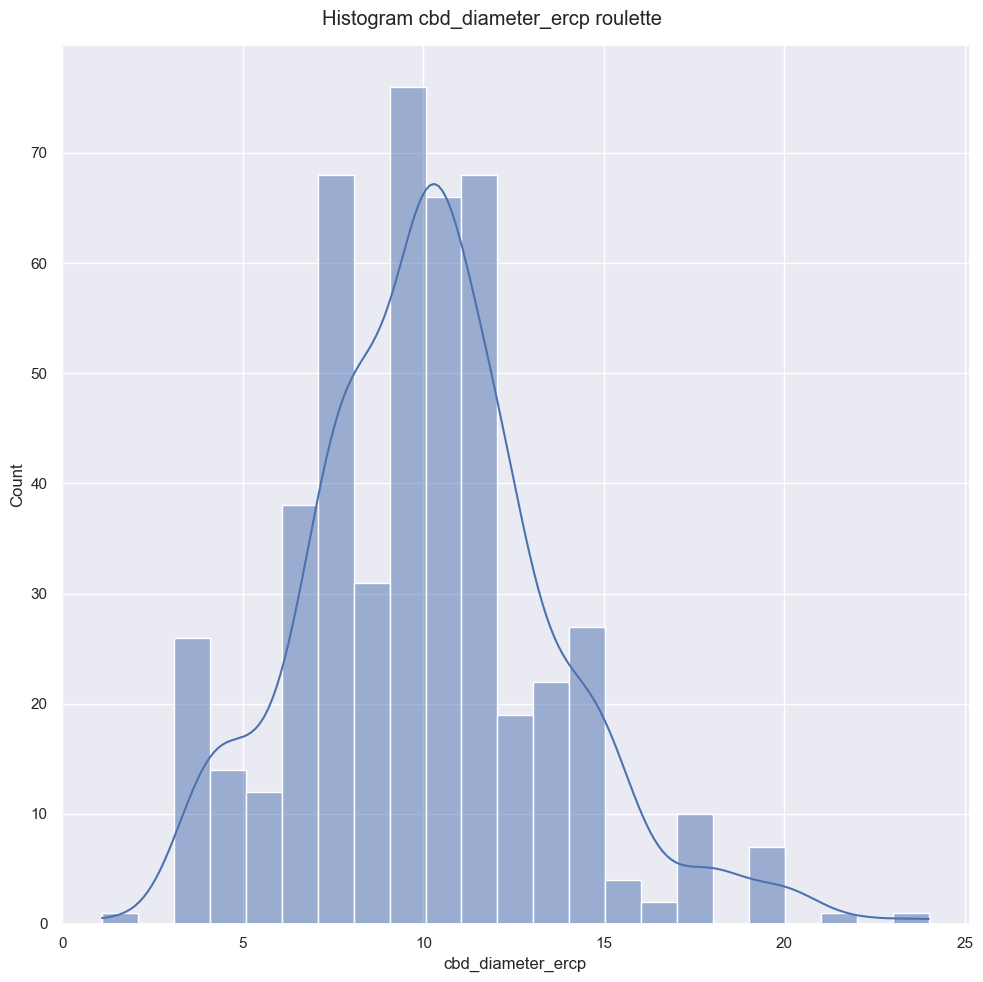
\includegraphics[width=\textwidth]{histogram_cbd_diameter_ercp_roulette}
		\caption{Histograma de atributo \emph{cbd\_diameter\_ercp} posterior a método de ruleta.}
	\end{subfigure}
	\caption{Resultados de datos sintéticos mediante el método ruleta}
	\label{Fig: roulette-hist}
\end{figure}


\FloatBarrier
\subsubsection{SMOTE}
La Figura \ref{Fig: SMOTE-class} muestra la distribución de clases resultante de aplicar el método SMOTE. La Tabla \ref{Tab: SMOTE-std} muestra una comparación entre la desviación estándar de los atributos de la base datos original y los datos obtenidos tras aplicar el método SMOTE. Por otro lado, la Figura \ref{Fig: smote-hist} muestra un ejemplo de la distribución de los datos resultantes del método SMOTE.

\begin{figure}[!htb]
	\centering
	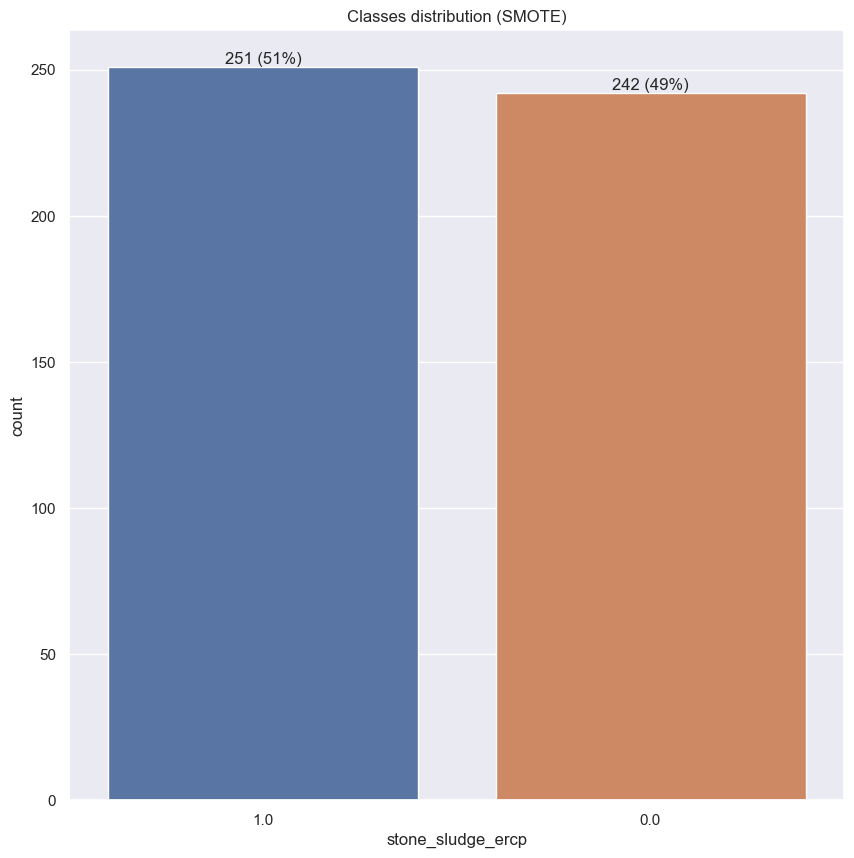
\includegraphics[width=0.7\textwidth]{classes_distribution_smote}
	\caption{Distribución de clases en el conjunto de datos resultante del método SMOTE}
	\label{Fig: SMOTE-class}
\end{figure}

\begin{table}[!htb]
\centering
\caption{Comparación de los valores de desviación estándar del conjunto de datos original y posterior al balance de clases por el método SMOTE.}
\label{Tab: SMOTE-std}
\begin{tabular}{|l|ll|}
\hline
\multicolumn{1}{|c|}{\multirow{2}{*}{\textbf{Atributo}}} & \multicolumn{2}{c|}{\textbf{$\sigma$}}                                           \\ \cline{2-3} 
\multicolumn{1}{|c|}{}                                   & \multicolumn{1}{c|}{\textbf{Original}} & \multicolumn{1}{c|}{\textbf{SMOTE}} \\ \hline
age\_at\_ercp                                            & \multicolumn{1}{l|}{17.81}             & 17.07                                \\ \hline
gender                                                   & \multicolumn{1}{l|}{0.48}              & 0.46                                 \\ \hline
race                                                     & \multicolumn{1}{l|}{1.19}              & 1.18                                 \\ \hline
bmi                                                      & \multicolumn{1}{l|}{7.47}              & 7.50                                 \\ \hline
parity                                                   & \multicolumn{1}{l|}{1.34}              & 1.15                                 \\ \hline
dm                                                       & \multicolumn{1}{l|}{0.36}              & 0.39                                 \\ \hline
ibd                                                      & \multicolumn{1}{l|}{0.05}              & 0.04                                 \\ \hline
cirrhosis                                                & \multicolumn{1}{l|}{0.18}              & 0.17                                 \\ \hline
peak\_bili                                               & \multicolumn{1}{l|}{19.73}             & 25.85                                \\ \hline
stones\_on\_bd                                           & \multicolumn{1}{l|}{1.10}              & 1.09                                 \\ \hline
cbd\_diameter\_us                                        & \multicolumn{1}{l|}{3.31}              & 3.14                                 \\ \hline
cbd\_diameter\_mrcp                                      & \multicolumn{1}{l|}{1.77}              & 1.54                                 \\ \hline
cbd\_diameter\_ercp                                      & \multicolumn{1}{l|}{3.34}              & 3.37                                 \\ \hline
intraductal\_filling                                     & \multicolumn{1}{l|}{0.94}              & 1.11                                 \\ \hline
cystic\_duct\_filling                                    & \multicolumn{1}{l|}{0.88}              & 0.87                                 \\ \hline
stone\_shape\_ercp                                       & \multicolumn{1}{l|}{0.87}              & 0.76                                 \\ \hline
stone\_color\_ercp                                       & \multicolumn{1}{l|}{1.31}              & 1.15                                 \\ \hline
pyobilia\_ercp                                           & \multicolumn{1}{l|}{0.87}              & 0.84                                 \\ \hline
gallbladder                                              & \multicolumn{1}{l|}{0.50}              & 0.48                                 \\ \hline
stone\_sludge\_ercp                                      & \multicolumn{1}{l|}{0.35}              & 0.50                                 \\ \hline
\end{tabular}
\end{table}

\begin{figure}[!htb]
	\centering
	\begin{subfigure}[b]{0.4\textwidth}
		\centering
		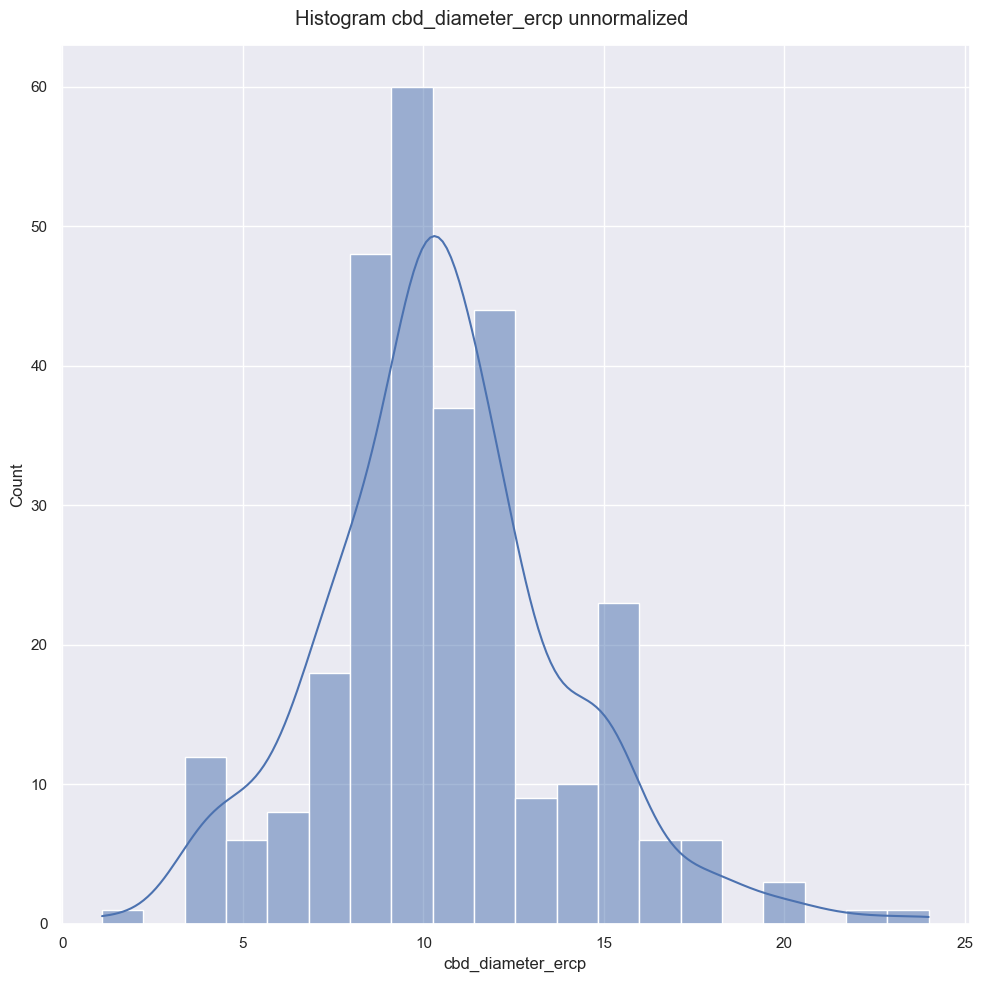
\includegraphics[width=\textwidth]{histogram_cbd_diameter_ercp_unnormalized}
		\caption{Histograma de atributo \emph{cbd\_diameter\_ercp} original.}
	\end{subfigure}
	\hfill
	\begin{subfigure}[b]{0.4\textwidth}
		\centering
		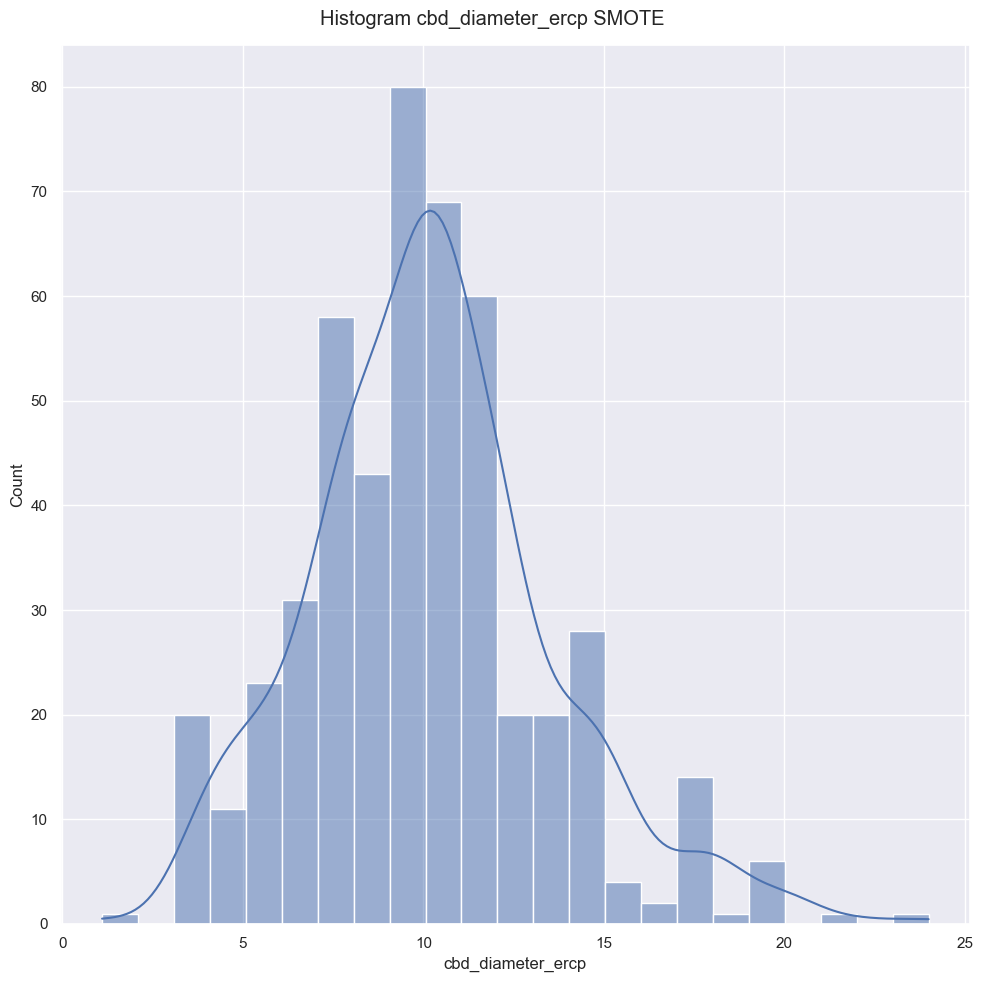
\includegraphics[width=\textwidth]{histogram_cbd_diameter_ercp_smote}
		\caption{Histograma de atributo \emph{cbd\_diameter\_ercp} posterior a método SMOTE.}
	\end{subfigure}
	\caption{Resultados de datos sintéticos mediante el método SMOTE}
	\label{Fig: smote-hist}
\end{figure}


\section{Conclusiones}
El manejo de datos faltantes siempre presenta un gran reto dentro del área de inteligencia artificial. Los métodos analizados e implementados en esta práctica han demostrado ser útiles para llenar estos espacios vacíos y no cambiar la distribución original de los datos.

Hablando específicamente de cada uno de los atributos trabajados tenemos:

\begin{itemize}
	\item \textbf{sex}. Dado a que solamente había 3 datos faltantes, fue bastante claro el implementar un método como la imputación por moda. Habría que investigar si dicho método es recomendable solamente ante ciertos rangos de datos faltantes.
	
	\item \textbf{hypertension}. Considerando que el índice de correlación máximo obtenido coincide con la variable objetivo, fue fácil imaginar que la imputación por media/moda de clases sería ideal, sin embargo al prestar atención al método podemos observar que la distribución de los posibles valores de este atributo es aproximadamente de 3:1, por lo que el método de moda de clase rellenó todos los faltantes con la clase 0, mismo resultado se hubiera obtenido con una imputación por moda y hubiera disminuido la complejidad computacional.
	
	\item \textbf{workt\_type y Residence\_type}. El método de imputación aleatoria logró mantener de forma adecuada la distribución de estas variables, comportamiento que se atribuye a la claras diferencias en la frecuencia de cada una de las observaciones de cada atributo, es muy probable que utilizar este método en atributos con mayor resolución no será eficaz.
	
	\item \textbf{bmi}. Considerar que el mayor índice de correlación fue con el atributo \emph{avg\_glucose\_level} fue de ayuda para lograr estimar una línea de tendencia entre ambos atributos, sin embargo, dicho valor de correlación apenas fue de $0.24$, lo cuál es un claro indicador de que no existe una relación lineal entre ambos atributos (afirmación que se confirma al generar un gráfico de dispersión entre ambos atributos (Figura \ref{Fig: Dispersion})). Existe la posibilidad de que utilizar algún tipo de regresión no lineal pueda mejorar el rendimiento de este método. A pesar de sus limitantes, es destacable el hecho de que se logró conservar la forma de la distribución de los datos originales.
\end{itemize}

\begin{figure}[htbp]
	\centering
	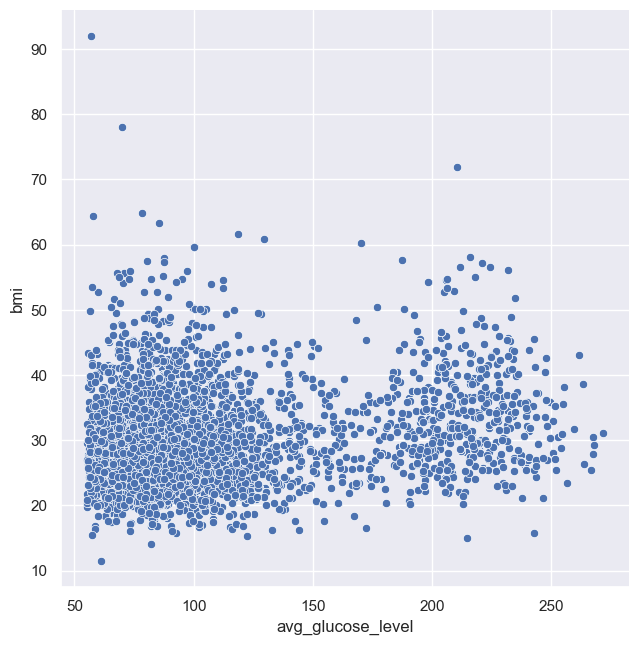
\includegraphics[width=0.8\textwidth]{bmi_glucose}
\end{figure}


\nocite{*}
\renewcommand{\refname}{Referencias bibliográficas}
\bibliographystyle{IEEEtran-spanish}
\bibliography{referencias}

\appendix
\section{Código documentado}
El código completo y funcional se puede encontrar anexo en el archivo \emph{zip} compartido en conjunto con este reporte, así como en las secciones anexas.

\subsection{Practica3\_EnriqueMenaCamilo.py}
Script implementado para el desarrollo de la práctica.
\inputminted[linenos=true, fontsize=\scriptsize]{Python}{../Practica3_EnriqueMenaCamilo.py}

\end{document}